\documentclass{article}

% --- Layout e formattazione generale ---
\usepackage[a4paper, landscape, twocolumn, margin=1.5cm, columnsep=1cm]{geometry}
\usepackage[hidelinks]{hyperref}

% --- Matematica ---
\usepackage{amsthm}
\usepackage{amsmath}
\usepackage{amsfonts}
\usepackage{amssymb}
\usepackage{xcolor}
\numberwithin{equation}{section}
\usepackage{mdframed}
\DeclareMathOperator*{\argmax}{arg\,max}
\DeclareMathOperator*{\argmin}{arg\,min}
\usepackage{cancel}

% --- Teoremi, definizioni e ambienti ---
\renewcommand\qedsymbol{$\blacksquare$}
\newtheorem*{definition}{\color{red}\textbf{Definition}}
\newtheorem*{theorem}{\color{green}\textbf{Theorem}}
\newtheorem*{proposition}{\color{blue}\textbf{Proposition}}
\newmdenv[%
    backgroundcolor=lightgray,
    frametitlebackgroundcolor=gray,
    hidealllines=true,
    frametitlefont=\sffamily\bfseries\color{white},
    frametitle={Example},
]{example}
\newmdenv[%
    backgroundcolor=yellow,
    hidealllines=true
]{recap}

% --- Grafica e disegni ---
\usepackage{graphicx}
\usepackage{wrapfig}
\graphicspath{ {./images/} }


\begin{document}
\pagenumbering{gobble}

\tableofcontents
\clearpage

\pagenumbering{arabic}
\parindent 0pt

\section{Linear Algebra Tools}
This chapter introduces inner product to give geometric meaning to vectors and
vector spaces, enabling calculations of length, distance, and angles.

\begin{definition}[Symmetric Positive Definitive Matrix] 
    A symmetric matrix $A\in \mathbb{R}^{n\times n}$ that satisfies
    \begin{equation}\label{positive_definite_matrix}
        \text{for every nonzero vector }x:x^TAx>0
    \end{equation}    
    is called \textbf{positive definite}. If only $\geq$ holds in
    \ref{positive_definite_matrix}, then $A$ is called \textbf{positive
    semidefinite}.
\end{definition}
These properties helps in identifying positive definite matrices without
having to check the definition explicitly:
\begin{enumerate}
    \item The null space of $A$ contains only the null vector; 
    \item The diagonal elements $a_{ii}$ of $A$ are positive; 
    \item The eigenvalues of $A$ are real and positive.
\end{enumerate}
\subsection{Angles and Orthogonality}
The angle $\omega$ between vectors $x$ and $y$ is computed as:
$$\cos\omega=\frac{\langle x,y\rangle}{\lVert x\rVert_2 \lVert y\rVert_2}$$ 
Here, $\langle x,y\rangle$ denotes the inner product between $x$ and $y$.

This angle indicated the vectors' similarity in orientation. 
\begin{definition}[Orthogonal vectors]
    Two vectors are orthogonal if $\langle x,y \rangle=0$. If additionally
    $\lVert x\rVert=1=\lVert y\rVert$, then $x$ and $y$ are orthonormal.
\end{definition}
\begin{definition}[Orthogonal matrix]
    A square matrix is an orthogonal matrix if and only if \underline{its columns are
    orthonormal} so that 
    $$AA^T=I=A^TA$$
    which implies that 
    $$A^{-1}=A^T$$
\end{definition}
The length of a vector $x$ is not changed when transforming it using an
orthogonal matrix $A$.
$$\lVert Ax\rVert_2^2=\lVert x\rVert_2^2$$
Moreover, the angle between any two vectors $x,y$ is also unchanged when
transforming both of them using an orthogonal matrix $A$.
\begin{definition}[Orthonormal Basis]
    In an $n$-dimensional vector space $V$ with a basis set
    $\{b_1,\ldots,b_n\}$, if all the basis vectors are orthogonal to each
    other, the basis is called as an \textbf{orthogonal basis}.
    Additionally, if the length of each basis vector is 1, the basis is
    referred to as an \textbf{orthonormal basis}.
\end{definition}
We can also have vector spaces that are orthogonal to each other. Given a
vector space $V$ of dimension $D$, let's  consider a subspace $U$ of dimension
$M$ such that $U\subseteq V$. Then its \textbf{orthogonal complement}
$U^{\perp}$ is a $D-M$ dimensional subspace $V$ and contains all vectors in
$V$ that are orthogonal to every vector in $U$.
\begin{center}
    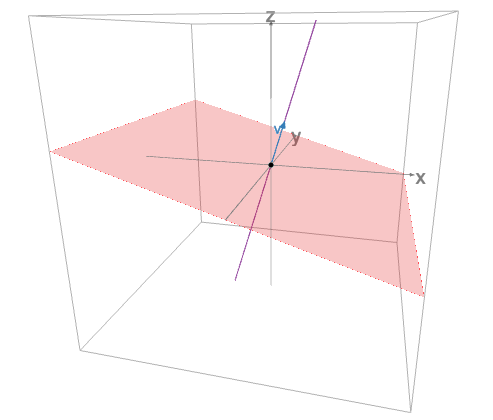
\includegraphics[width=0.6\linewidth]{images/orthogonal_complement}
\end{center}
\subsubsection{Orthogonal Projections}
Projections are key linear transformations in machine learning and are
particularly useful for handling high-dimensional data. Often, only a few
dimensions in such data are essential for capturing the most relevant
information. By projecting the original high-dimensional data onto a lower
dimensional feature space, we can work more efficiently to learn about the
dataset and extract significant patterns.
\begin{definition}[Projection]
    Let $V$ be a vector space and $U\subseteq V$ a subspace of $V$. A linear
    mapping $\pi:V\to U$ is called \textbf{projection} if it satisfies
    $\pi^2=\pi\circ\pi=\pi$.
\end{definition}
Given that linear mappings can be represented by transformation matrices, the
above definition extends naturally to \textit{projection matrices} $P_{\pi}$.
These matrices exhibit the property that $P_{\pi}^2=P_{\pi}$.

The projection $\pi_U(x)$ of a vector $x\in \mathbb{R}^n$ onto a subspace $U$
is the closest point necessarily in $U$ to $x$.
\cleardoublepage
\section{Matrix Decompositions}
\subsection{Eigenvalues and Eigenvectors}
Eigenanalysis helps us understand linear transformations represented by a
matrix $A$. Eigenvectors $x$ are special vectors that only get scaled, not
rotated, when multiplied by $A$. The scaling factor is the eigenvalue
$\lambda$, which indicated how much $x$ is stretched or shrunk. $\lambda$ can
also be zero.
\begin{definition}[Eigenvalue and Eigenvector]
    Let $A\in \mathbb{R}^{n\times n}$ be a square matrix. Then $\lambda\in
    \mathbb{R}$ is an \textbf{eigenvalue} of $A$ and nonzero vector $x$ is the
    corresponding \textbf{eigenvector} of $A$ if 
    \begin{equation}\label{eq:eigenvalue_equation}
        Ax=\lambda x
    \end{equation}
    We call \ref{eq:eigenvalue_equation} the \textbf{eigenvalue equation}.
\end{definition}
The following statements are equivalent:
\begin{itemize}
    \item $\lambda$ is an eigenvalue of $A\in \mathbb{R}^{n\times n}$.
    \item A nonzero vector $x$ exists such that $Ax=\lambda x$ or,
        equivalently, $(A-\lambda I_n)x=0$ for $x\neq 0$.
    \item Then $A-\lambda I$ is a \textbf{singular
        matrix} and its determinant is \textbf{zero}.
\end{itemize}
Each eigenvector $x$ has one unique eigenvalue $\lambda$, but each $\lambda$
can have multiple eigenvectors.
\begin{definition}[Eigenspace and Eigenspectrum]
    For $A\in \mathbb{R}^{n\times n}$, the set of all eigenvectors of $A$
    associated with an eigenvalue $\lambda$ spans a subspace of
    $\mathbb{R}^n$, which is called the \textbf{eigenspace} of $A$ with
    respect to $\lambda$ and is denoted by $E_{\lambda}$. The set of all
    eigenvalues of $A$ is called the \textbf{eigenspectrum} of $A$.
\end{definition}
\begin{definition}
    Let $\lambda_i$ be an eigenvalue of a square matrix $A$. Then the
    \textbf{geometric multiplicity} of $\lambda_i$ is the number of linearly
    independent eigenvectors associated with $\lambda_{i}$. In other words, it
    is the dimensionality of the eigenspace spanned by the eigenvectors
    associated with $\lambda_i$.
\end{definition}
\begin{theorem}
    The eigenvectors $x_1,\ldots,x_n$ of a matrix $A\in \mathbb{R}^{n\times
    n}$ with $n$ distinct eigenvalues $\lambda_1,\ldots,\lambda_n$ are
    linearly independent.
\end{theorem}
This theorem states that eigenvectors of a matrix with $n$ distinct eigenvalues
form a basis of $\mathbb{R}^n$.
\cleardoublepage
\section{Least Square Problem}
Considering the problem 
$$\underset{m\times n}{A}x=b$$
with more rows than columns ($m>n$).

Finding an exact solution to this system, i.e. satisfying $Ax-b=0$ is
impossible. However, we can seek an approximate solution $\tilde{x}$, such
that $A\tilde{x}-b\approx0$.

To quantify the closeness of the vector $A\tilde{x}-b$, also called residual
, to zero, we use the 2-norm. Thus,
$$\tilde{x}=\argmin_{x\in \mathbb{R}^n}\lVert Ax-b\rVert_2$$
This minimization problem can be expressed in terms of the squared 2-norm,
which is equivalent:
$$\tilde{x}=\argmin_{x\in \mathbb{R}^n}\lVert Ax-b\rVert_2^2$$

Considering the $r=\text{rank}(A)$ we have two possibilities:
\begin{enumerate}
    \item $r=n\to$ The least square problem has a unique solution $\forall b\in
        \mathbb{R}^m$.

        By solving the so-called \textbf{normal equations}
        $$A^TAx=A^Tb$$
        where $A^TA$ is $n\times n$ symmetric and positive definite matrix if
        $\text{rank}(A)=n$ then the matrix is non singular. This can be
        computed efficiently using the direct method \textsc{Cholesky
        decomposition}.

        For any $B$ symmetric and positive definite, the Cholesky decomposition
        factorizes it as the product of two matrices:
        $$B=LL^T$$
        where $L$ is lower triangular and $L^T$ is upper triangular.

        The computational complexity is $\mathcal{O}(\frac{n^3}{6})$, which is
        half of complexity of LU factorization.

        The solution $x$ is then computed as
        $$
        \begin{aligned}
            A^TAx=A^Tb\\
            L\underbrace{L^Tx}_{y}=A^Tb\\
            \begin{cases}
                Ly=A^Tb \\ 
                L^Tx=y
            \end{cases}
        \end{aligned}
        $$
    \item $r<n\to$ The least square problem has infinite solutions $\forall
        b\in \mathbb{R}^m$.

        Among the infinite possible solutions $S=\{x\in\mathbb{R}^n\ |\
        x\text{ solutions of } \min\lVert Ax-b\rVert_2^2\}$ we are interested
        in  computing one \underline{unique} $x^*$ that has the minimum norm
        (2-norm): 
        $$x^*=\min_{x\in S}\lVert x \rVert_2$$
        That is computed using the SVD decomposition of $A=U\Sigma V^T$:
        $$x^*=\sum_{i=1}^r\frac{u_i^Tb}{\sigma_i}v_i$$
        where $U=(u_1,\ldots,u_m)\in\mathbb{R}^{m\times m}$,
        $V=(v_1,\ldots,v_n)\in\mathbb{R}^{n\times n}$, $\sigma_i\in\mathbb{R}^+$ and
        $b\in\mathbb{R}^m$.
\end{enumerate}
\begin{example}
    Consider a polynomial of degree $n$ given by
    $f_\theta(x)=\theta_0+\ldots+\theta_nx^n$, where we want compute the
    parameters $\theta=\{\theta_0,\ldots,\theta_n\}$ that fit well the given
    data pairs $(x_i,y_i)_{i=0,\ldots,m}$.
    \begin{center}
        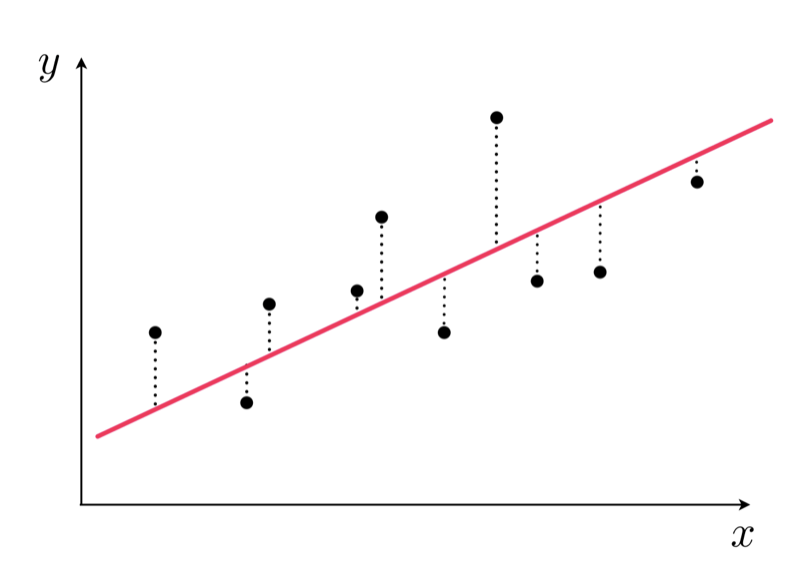
\includegraphics[width=0.5\linewidth]{least_square}
    \end{center}
    Fitting the data means to minimize the residuals (the distance between an
    observed value and the predictor's value) $r=(r_0,\ldots,r_m)=y-Ax-b$,
    through the solution of a least square problem. In this context, $Ax-b$ is
    defined as follows:
    $$
    \begin{cases}
        r_0=y_0-f(x_0)=y_0-(\theta_0+\ldots+\theta_nx_0^n)\\
        \vdots \\ 
        r_m=y_m-f(x_m)=y_m-(\theta_0+\ldots+\theta_nx_m^n)\\
    \end{cases}
    $$
    This expression can be more compactly rewritten as $r=y-A\theta$ where $A$
    is given by:
    $$A=\begin{bmatrix}
        1 & x_0 & x_0^2 & \ldots & x_0^n \\
        1 & x_1 & x_1^2 & \ldots & x_1^n \\
        \vdots & \vdots & \vdots & & \vdots \\
        1 & x_m & x_m^2 & \ldots & x_m^n \\
    \end{bmatrix}$$
    Therefore, the task of minimizing $r$ can be formulated as:
    $$\min_{\theta\in\mathbb{R}^n}\lVert y-A\theta\rVert_2^2$$
\end{example}
\cleardoublepage
\section{Vector calculus}
Firstly, we'll explore partial derivatives and gradients, focusing on functions that take a vector as input and produce a
single real number as output. These functions are formally represented as
$f:\mathbb{R}^n\to \mathbb{R}$.

Subsequently, we will extend these ideas to functions that not only take a
vector as input but also produce a vector as output. These functions can be
written as $f:\mathbb{R}^n\to \mathbb{R}^m$.

\subsection{Gradients of Real-Valued Functions}
When we deal with a function that depends on multiple variables, such as 
$f(x)=f(x_1,x_2)$, we use the \textbf{gradient} to represent its derivative.
The gradient is a vector composed of \textbf{partial derivates} of the
function. To compute each partial derivates, we differentiate the function
with respect to one variable while keeping all other variables constant.
\begin{equation}\label{eq:gradient_real_valued_functions}
   \nabla_x f=\begin{bmatrix}
       \frac{\partial{f}}{\partial{x_1}} &
       \frac{\partial{f}}{\partial{x_2}} & \cdots &
       \frac{\partial{f}}{\partial{x_n}}
    \end{bmatrix}\in \mathbb{R}^{1\times n} 
\end{equation}
where $n$ is the number of variables.
\paragraph{Basic Rules of Partial Differentiation}
\begin{itemize}
    \item[] Product rule:
        $$\frac{\partial}{\partial{x}}(f(x)g(x))=\frac{\partial{f}}{\partial{x}}g(x)+f(x)\frac{\partial{g}}{\partial{x}}$$
    \item[] Sum rule:
        $$\frac{\partial}{\partial{x}}(f(x)+g(x))=\frac{\partial{f}}{\partial{x}}+\frac{\partial{g}}{\partial{x}}$$
    \item [] Chain rule:
        $$\frac{\partial}{\partial{x}}(g\circ
        f)(x)=\frac{\partial}{\partial{x}}\left(g(f(x))\right)=\frac{\partial{g}}{\partial{f}}\frac{\partial{f}}{\partial{x}}$$
\end{itemize}

In the context of the chain rule, consider $f$ as implicitly a composition
$f\circ g$.

If a function $f(x_1,x_2)$ is a function of $x_1$ and $x_2$, where
$x_1(t)$ and $x_2(t)$ are themselves functions of a single variable $t$, the
chain rule yields the partial derivates
$$\frac{\text{d}f}{\text{d}t}=\begin{bmatrix}
    \frac{\partial{f}}{\partial{x_1}} & \frac{\partial{f}}{\partial{x_2}}
    \end{bmatrix}\begin{bmatrix}
    \frac{\partial{x_1(t)}}{\partial{t}} \\ 
    \frac{\partial{x_2(t)}}{\partial{t}}
\end{bmatrix}=\frac{\partial{f}}{\partial{x_1}}\frac{\partial{x_1}}{\partial{t}}+\frac{\partial{f}}{\partial{x_2}}\frac{\partial{x_2}}{\partial{t}}$$
\newpage
\begin{example}
    Consider $f(x_1,x_2)=x_1^2+2x_2$, where $x_1=\sin t$ and $x_2=\cos t$,
    then
    $$\text{with}\quad\frac{\partial{f}}{\partial{x_1}}=2x_1,\quad \frac{\partial{f}}{\partial{x_2}}=2$$
    $$\begin{aligned}
        \frac{\text{d}f}{\text{d}t}&=2\sin t \frac{\partial{\sin t}}{\partial{t}}+2 \frac{\partial{\cos
        t}}{\partial t}\\
            &=2\sin t\cos t-2\sin t
    \end{aligned}$$
\end{example}
If a function $f(x_1,x_2)$ is a function of $x_1$ and $x_2$, where $x_1(s,t)$
and $x_2(s,t)$ are themselves functions of two variables $s$ and $t$, the
chain rule yields the partial derivates
$$
\frac{\text{d}f}{\text{d}(s,t)}=\begin{bmatrix}
    \frac{\partial{f}}{\partial{s}} & \frac{\partial{f}}{\partial{t}}
\end{bmatrix} 
$$
where 
$$
\begin{aligned}
    \frac{\partial{f}}{\partial{s}}&=\frac{\partial{f}}{\partial{x_1}}\frac{\partial{x_1}}{\partial{{\color{red}s}}}+\frac{\partial{f}}{\partial{x_2}}\frac{\partial{x_2}}{\partial{{\color{red}s}}}\\
    \frac{\partial{f}}{\partial{t}}&=\frac{\partial{f}}{\partial{x_1}}\frac{\partial{x_1}}{\partial{{\color{blue}t}}}+\frac{\partial{f}}{\partial{x_2}}\frac{\partial{x_2}}{\partial{{\color{blue}t}}}\\
\end{aligned}
$$
Another way to obtain these two partial derivatives is to represent the
previous formula as a row vector containing the partial derivatives of $f$
with respect to $x_1$ and $x_2$. This row vector is then multiplied by a
matrix composed of the partial derivatives of $x_1$ and $x_2$ with respect to
$s$ and $t$. When you perform this multiplication, you get the exact same
result as above.
$$
\begin{bmatrix}
    \frac{\partial{f}}{\partial{s}} & \frac{\partial{f}}{\partial{t}}
\end{bmatrix}=\begin{bmatrix}
    \frac{\partial{f}}{\color{red}\partial{x_1}} &
    \frac{\partial{f}}{\color{blue}\partial{x_2}}
\end{bmatrix}\begin{bmatrix}
    {\color{red}\frac{\partial{x_1}}{\partial{s}}} &
    {\color{red}\frac{\partial{x_1}}{\partial{t}}} \\ 
    {\color{blue}\frac{\partial{x_2}}{\partial{s}}} &
    {\color{blue}\frac{\partial{x_2}}{\partial{t}}}
\end{bmatrix}$$
\newpage
\begin{example}
    Given the following functions:\\
    $g:\mathbb{R}^2\to \mathbb{R}^2\quad g(s,t)=(\sin(t)s, \cos(s)t)$\\ 
    $f:\mathbb{R}^2\to \mathbb{R}\quad f(x_1,x_2)=x_1^2+2x_2$\\ 
    $f\circ g: \mathbb{R}^2\to \mathbb{R}$\\
    Compute $\nabla_{(s,t)}(f\circ g)$ and evaluate $\nabla_{(s,t)}(f\circ g)(0,0)$.
    $$
    \begin{aligned}
        &=\begin{bmatrix}
            2s\sin(t) & 2
        \end{bmatrix}
        \begin{bmatrix}
            \sin(t) & s\cos(t)\\ 
            -t\sin(s) & \cos(s)
        \end{bmatrix} \\ 
        &=\begin{bmatrix}
            2s\sin^2(t)-2t\sin(s) \\ 
            2s^2\sin(t)\cos(t)+2\cos(s)
        \end{bmatrix}=(0,2)
    \end{aligned}
    $$
\end{example}
\subsection{Gradients of Vector-Valued Functions}
We can express a vector-valued function $f:\mathbb{R}^n\to \mathbb{R}^m$ as a
column vector of $m$ real-valued functions $f_i:\mathbb{R}^n\to \mathbb{R}$.
Given an input vector $x=\begin{bmatrix} x_1,\ldots,x_n \end{bmatrix}^T\in
\mathbb{R}^n$, the output is defined as: 
$$
f(x)=\begin{bmatrix} f_1(x)\\
\vdots \\ f_m(x) \end{bmatrix}\in \mathbb{R}^m
$$
\begin{definition}[Jacobian]
    By contrast, in Equation \ref{eq:gradient_real_valued_functions}, each partial
    derivative $\frac{\partial f}{\partial x_i}$ is a column vector.
    $$
    \begin{aligned}
        J=\nabla_x f&=\begin{bmatrix}
            \frac{\partial{f}}{\partial{x_1}} & \cdots &
            \frac{\partial{f}}{\partial{x_n}}
        \end{bmatrix} \\ 
                  &=\begin{bmatrix}
                      \frac{\partial{f_1}}{\partial{x_1}} & \cdots &
                      \frac{\partial{f_1}}{\partial{x_n}} \\ 
                      \vdots & & \vdots \\ 
                      \frac{\partial{f_m}}{\partial{x_1}} & \cdots &
                      \frac{\partial{f_m}}{\partial{x_n}} \\ 
                  \end{bmatrix}\\
            J(i,j)&=\frac{\partial f_i}{\partial{x_j}}
    \end{aligned}
    $$
    The collection of all first-order partial derivatives of a vector-valued
    function $f:\mathbb{R}^n\to \mathbb{R}^m$ is called the \textbf{Jacobian}.
    The Jacobian $J$ is an $m\times n$ matrix.
\end{definition}
\begin{definition}[Hessian]
    The \textbf{Hessian}, denoted as $\nabla_{x_i,x_j}^2$, is the collection
    of all second-order derivatives and the corresponding \textbf{Hessian
    matrix}
    $$H=\begin{bmatrix}
        \frac{\partial^2f}{\partial x_1^2} & \ldots & \frac{\partial^2f}{\partial
        x_1\partial x_n} \\ 
        \vdots & \ddots & \vdots \\ 
        \frac{\partial^2f}{\partial x_n\partial x_1} & \ldots &
        \frac{\partial^2f}{\partial x_n^2} \\ 
    \end{bmatrix}\in\mathbb{R}^{n\times n}$$
    is symmetric. The element at position $i,j$ is defined as
    $\frac{\partial^2f}{\partial x_ix\partial x_j}$.
\end{definition}
\begin{example}
    $f:\mathbb{R}^2\to \mathbb{R}^3,\quad f:(x_1,x_2)=\begin{pmatrix}
        x_1+x_2 \\ 
        2x_1^2-x_2 \\ 
        -x_1x_2
    \end{pmatrix}$\\ 
    $J(f):\mathbb{R}^2\to \mathbb{R}^{3\times 2},\quad J(i,j)=\begin{bmatrix}
        1 & 1 \\ 
        4x_1 & -1 \\ 
        -x_2 & -x_1 
    \end{bmatrix},\quad
    J(1,1)=\begin{bmatrix}
        1 & 1 \\ 
        4 & -1 \\ 
        -1 & -1
    \end{bmatrix}$
\end{example}
\begin{example}
   Let us consider the linear model 
   $$y=\Phi\theta$$
   where $\theta\in \mathbb{R}^D$ is a parameter vector, $\Phi\in
   \mathbb{R}^{N\times D}$ are input features, and $y\in \mathbb{R}^N$ are the
   corresponding observations. We define the functions 
   $$\begin{aligned}
       e:\mathbb{R}^D\to \mathbb{R}^N,\quad e(\theta)&=y-\Phi\theta \\
       L:\mathbb{R}^N\to \mathbb{R},\quad L(e)&=\lVert e\rVert_2^2, \quad
       L(\theta)= \lVert y-\Phi\theta\rVert_2^2
   \end{aligned}$$
   This is called a \textbf{least-squares loss} function.\\ We want to find
   $\frac{\partial{L}}{\partial{\theta}}$, which is derivative of the loss
   function with respect to the parameters $\theta$. This will allow us to
   find the optimal $\theta$ that minimizes the loss function $L(\theta)$.

   The chain rule allows us to compute the gradient as 
   $$\frac{\partial{L}}{\partial{e}}={\color{red}\frac{\partial{L}}{\partial{e}}}{\color{blue}\frac{\partial{e}}{\partial{\theta}}}$$
   We know that $\lVert e\rVert_2^2=e^Te$ and so 
   $${\color{red}\frac{\partial{L}}{\partial{e}}=2e^T}\in \mathbb{R}^{1\times
   N}$$
   Furthermore, we obtain 
   $${\color{blue}\frac{\partial{e}}{\partial{\theta}}=-\Phi}\in
   \mathbb{R}^{N\times D}$$
   such that our desired derivative is
   $$
   \nabla{L}_{\theta}=-2e^T\Phi=-2\underbrace{\color{red}(y^T-\theta^T\Phi^T)}_{1\times
   N}\underbrace{\color{blue}\Phi}_{N\times D}\in \mathbb{R}^{1\times D}\\ 
   $$
\end{example}
\subsection{Backpropagation and Automatic Differentiation}
In machine learning, finding optimal model parameters often involves
performing gradient descent. This requires computing the gradient of a
learning objective with respect to the model's parameters. Calculating the
gradient explicitly can be impractical due to the complexity and length of the
resulting derivative equations. To address this, the \textbf{backpropagation} algorithm
was introduced in 1962 as an efficient way to compute these gradients,
particularly for neural networks.

In neural networks, the output $y$ is computed through a multi-layered
function composition $y=(f_K\circ f_{K-1}\circ \cdots f_1)(x)$. Here, $x$ are
the inputs (e.g., images), $y$ are the observations (e.g., class labels).
Each functions $f_i,i=1,\ldots,K$, has its own parameters.
Specifically, in the $i^{th}$ layer, the function is given
$f_i(x_{i-1})=\sigma(A_{i-1}+b_{i-1})$, where $x_{i-1}$ is
the output from layer $i-1$ and $\sigma$ is an activation function. 
\begin{center}
    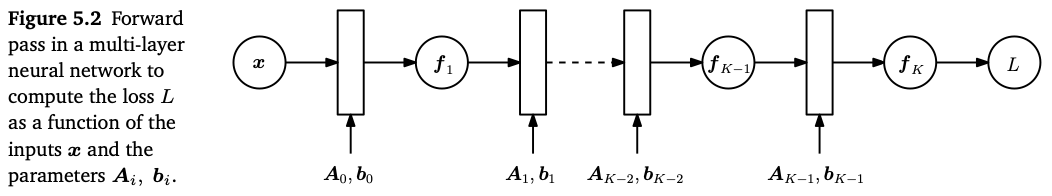
\includegraphics[width=\linewidth]{nn_forward_pass}
\end{center}
In order to train a neural network, we aim to minimize a loss function $L$
with respect to all parameters $A_j,b_j$ for $j=0,\ldots,K-1$.
Specifically, we're interested in optimizing these parameters to minimize the
squared loss given by
$$L(\theta)=\lVert y-f_K(\theta,x)\rVert^2$$
where $\theta=\{A_0, b_0, \ldots,A_{K-1},b_{K-1}\}$.

To minimize $L(\theta)$ we need to compute its gradients of $L$ to the
parameter set $\theta$. This involes calculating the partial derivatives of
$L$ with respect to the parameters $\theta_j=\left\{A_j,b_j\right\}$ for each
layer $j=0,\ldots,K-1$. The chain rule allows us to determine the partial
derivatives as
$$\begin{aligned}
    \frac{\partial{L}}{\partial{\theta_{K-1}}}&=\frac{\partial{L}}{\partial{f_K}}{\color{blue}\frac{\partial{f_K}}{\partial{\theta_{K-1}}}}
    \\
    \frac{\partial{L}}{\partial{\theta_{K-2}}}&=\frac{\partial{L}}{\partial{f_K}}\boxed{{\color{red}\frac{\partial{f_K}}{\partial{f_{K-1}}}}{\color{blue}\frac{\partial{f_{K-1}}}{\partial{\theta_{K-2}}}}}
    \\
    \frac{\partial{L}}{\partial{\theta_{K-3}}}&=\frac{\partial{L}}{\partial{f_K}}{\color{red}\frac{\partial{f_K}}{\partial{f_{K-1}}}}\boxed{{\color{red}\frac{\partial{f_{K-1}}}{\partial{f_{K-2}}}}{\color{blue}\frac{\partial{f_{K-2}}}{\partial{\theta_{K-3}}}}}
    \\
    \frac{\partial{L}}{\partial{\theta_{i}}}&=\frac{\partial{L}}{\partial{f_K}}{\color{red}\frac{\partial{f_K}}{\partial{f_{K-1}}}\cdots}\boxed{{\color{red}\frac{\partial{f_{i+2}}}{\partial{f_{i+1}}}}{\color{blue}\frac{\partial{f_{i+1}}}{\partial{\theta_{i}}}}}
\end{aligned}$$
The {\color{red}red} terms are partial derivatives of the output of a layer
with respect to its inputs, whereas the {\color{blue}blue} terms are partial
derivatives of the output of a layer with respect to its parameters. The
additional terms that we need to compute are indicated by the \fbox{boxes}.

The key insight of backpropagation is to reuse previously computed derivatives
to avoid redundant calculations. When we've computed the partial derivatives
$\frac{\partial{L}}{\partial{\theta_{i+1}}}$, we can reuse them to efficiently
calculate the partial derivatives
$\frac{\partial{L}}{\partial{\theta}_{i}}$.

It turns out that backpropagation is a special case of a set of techniques
known as \textbf{automatic differentiation}. Automatic differentiation
numerically evaluate the exact (up to machine precision) gradient of a function by working with
intermediate variables and applying the chain rule.

\begin{center}
    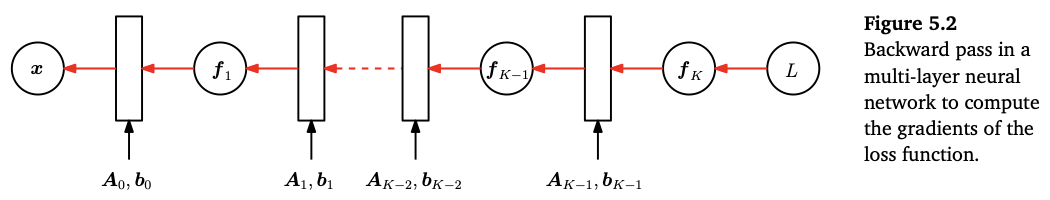
\includegraphics[width=\linewidth]{nn_backward_pass}
\end{center}
\begin{example}
    Consider the real-valued function 
    $$f(x)=\sqrt{x^2+\exp(x^2)}+\cos(x^2+\exp(x^2))$$
    Another way to attach this would be to just define some \textit{intermediate
    variables}. Say 
    $$
    \begin{aligned}
        a=x^2\\
        b=\exp(a)\\ 
        c=a+b\\ 
        d=\sqrt{c}\\ 
        e=\cos(c)\\ 
        f=d+e
    \end{aligned}
    $$
    The set of equations that include intermediate variables can be thought of
    as a computational graph 
    \begin{center}
        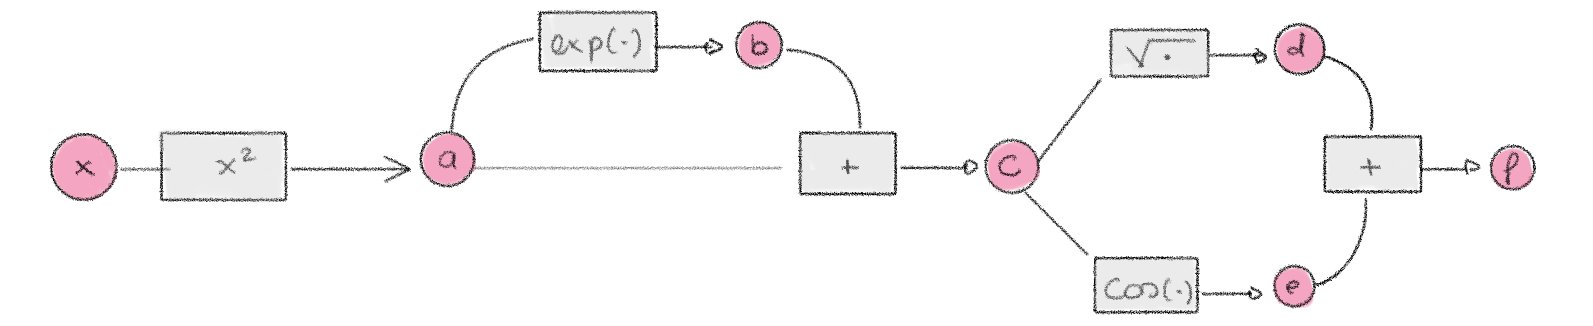
\includegraphics[width=\linewidth]{nn_backpropagation}
    \end{center}
    By looking at the computation graph, we can compute
    $\frac{\partial{f}}{\partial{x}}$ by working backward from the end of the
    graph and obtain the derivative of each variable, making the use of the
    derivatives of the children of that variable
    $$\begin{aligned}
        \frac{\partial{f}}{\partial{d}}=\frac{\partial{f}}{\partial{e}}=1 \\
        \frac{\partial{f}}{\partial{c}}=\frac{\partial{f}}{\partial{d}}\frac{\partial{d}}{\partial{c}}+\frac{\partial{f}}{\partial{e}}\frac{\partial{e}}{\partial{c}}
        \\ 
        \frac{\partial{f}}{\partial{b}}=\frac{\partial{f}}{\partial{c}}\frac{\partial{c}}{\partial{b}}
        \\
        \frac{\partial{f}}{\partial{a}}=\frac{\partial{f}}{\partial{b}}\frac{\partial{b}}{\partial{a}}+\frac{\partial{f}}{\partial{c}}\frac{\partial{c}}{\partial{a}}
        \\ 
        \frac{\partial{f}}{\partial{x}}=\frac{\partial{f}}{\partial{a}}\frac{\partial{a}}{\partial{x}}
    \end{aligned}$$
    We observe that the computation required for calculating the derivative is
    of similar complexity as the computation of the function itself (forward
    pass).
\end{example}
Automatic differentiation is a formalization of last Example. Let
$x_1,\ldots,x_d$ be the input variables to the function,
$x_{d+1},\ldots,x_{D-1}$ be the intermediate variables, and $x_D$ the output
variable. Then the computation graph can be expressed as follows:
\begin{equation}\label{eq:forward_pass}
    \text{For }i=d+1,\ldots,D:\quad x_i=g_i(x_{Pa}(x_i))
\end{equation}
where the $g_i(\cdot)$ are elementary functions and $x_{Pa}(x_i)$ are the
parent nodes of the variable $x_i$ in the graph.

Recall that by definition $f=x_D$ and hence
$$\frac{\partial{f}}{\partial{x_D}}=1$$
For other variables $x_i$, we apply the chain rule 
\begin{equation}\label{eq:backward_pass}
    \frac{\partial{f}}{\partial{x_i}}=\displaystyle\sum_{x_j:x_i\in
    Pa(x_j)}\frac{\partial{f}}{\partial{x_j}}\frac{\partial{x_j}}{\partial{x_i}}=\displaystyle\sum_{x_j:x_i\in
    Pa(x_j)}\frac{\partial{f}}{\partial{x_j}}\frac{\partial{g_j}}{\partial{x_i}}
\end{equation}
where $Pa(x_j)$ is the set of parent nodes of $x_j$ in the computation graph.
In other words, we apply the chain rule to any node for which $x_i$ is a
parent, and so on. Equation \ref{eq:forward_pass} is the \underline{forward
pass}, whereas \ref{eq:backward_pass} is the \underline{backward pass}.

The automatic differentiation approach works whenever we have a function that
can be expressed as a computation graph, where the elementary functions are
differentiable. 
\cleardoublepage
\section{Continuous Optimization}
Training a machine learning essentially involves identifying a good set of
parameters. What constitutes ``good'' is defined by the objective function.
Optimization algorithms are employed to locate the best possible value of this
function. Typically, the aim is to minimize the objective function, implying
that the best value is the minimum one.

\begin{figure}[!h]
   \centering
   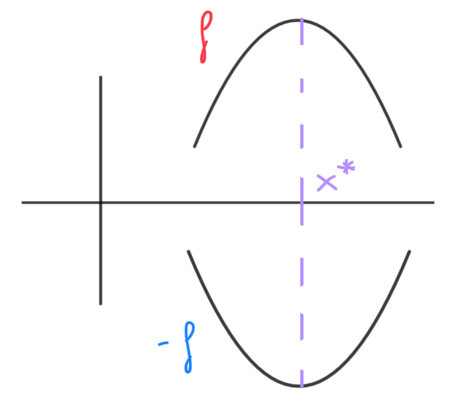
\includegraphics[width=0.25\linewidth]{argmin_argmax}
   \caption{$\underset{x\in \mathbb{R}^n}\argmax\
   f(x)=\underset{x\in\mathbb{R}^n}\argmin\ {-f(x)}$}
\end{figure}

We will assume in this chapter that our objective function $f:\mathbb{R}^n\to
\mathbb{R}$ is differentiable, hence we have access to a gradient to help us
find the optimal value. Intuitively, finding the best value is like finding
the valleys of the objective function, and the gradients point us uphill. The
idea is to move downhill (opposite to the gradient) and hope to find the
deepest point.
\subsection{Conditions for the existence of the minimum} 
\begin{definition}
    $f$ is differentiable if the partial derivates
    $\frac{\partial{f}}{\partial{x_i}},i=1,\ldots,n$ exist and are continuous. 
\end{definition}
\begin{definition}
    $x^*\in \mathbb{R}^n$ is a (strict) \textbf{local minimum} of $f$ if there
    exists $\epsilon>0$ such that:
    $$f(x^*)(<)\leq f(x)\quad \forall x: \lVert x-x^*\rVert<\epsilon$$
\end{definition}
\begin{definition}
    $x^*\in \mathbb{R}^n$ is a (strict) \textbf{global minimum} of $f$ if 
    $$f(x^*)(<)\leq f(x)\quad \forall x\in\mathbb{R}^N$$
\end{definition}
\begin{center}
    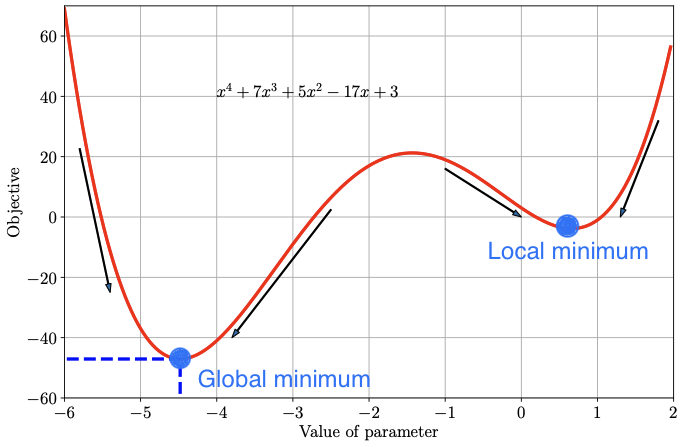
\includegraphics[width=0.75\linewidth]{local_global_minimum}
\end{center}
\begin{definition}[First order conditions]
    If $x^*$ is a minimum point of $f$, then $\nabla f(x^*)=0$. Furthermore,
    if $\nabla f(x^*)=0$ for $x^*\in \mathbb{R}^n$, then $x^*$ can be either a
    (local) minimum, a (local) maximum or a saddle point of $f(x)$.
\end{definition}
Consequently, we want to find a point $x^*\in \mathbb{R}^n$ such that $\nabla
f(x^*)=0$. Those points are stationary points for $f$.
\begin{center}
    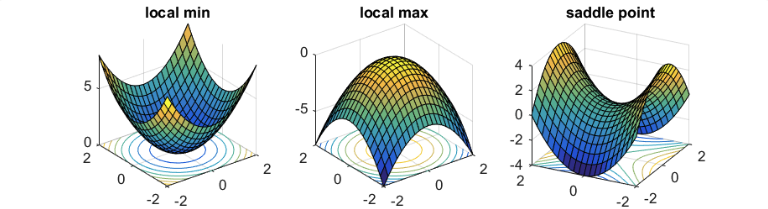
\includegraphics[width=\linewidth]{min_max_saddle}
\end{center}
\begin{definition}[Second order conditions]
    if $f$ is twice differentiable and if $\nabla f(x^*)=0$ and
    $\nabla^2f(x^*)$ (the hessian of $f$) is positive definitive then $x^*$ is
    a strict local minimum for $f$.
\end{definition}
\subsection{Algorithm to compute the minimum}

\paragraph{Iterative methods.} Given an initial vector $x_0\in \mathbb{R}^n$,
it is possible to approximate a solution to a given optimization problem by
applying iterative methods. In particular, by using these methods, one can
compute $x_{k+1}$ as follows:
$$x_{k+1}=g(x_k)$$
until convergence. In this case $g$ is an arbitrary function. Using these
methods, $x_k\to x^*$ for $k\to\infty$, where $x^*$ is a stationary point.

\paragraph{Descent methods} are iterative methods in which one can compute
$x_{k+1}$ as follows:
$$x_{k+1}=x_k+\alpha_kp_k$$
where $p_k\in \mathbb{R}^n$ and $\alpha_k\in \mathbb{R}$.
\begin{definition}
    $p_k$ is called a \textbf{descent direction} for $f$ in $x$ if there
    exists $\alpha_k>0$ such that:
    $$f(x_k+\alpha_k p_k)<f(x_k)$$
    In this case:
    $$p_k^T\nabla f(x_k)<0\quad\text{if } p\neq0$$
    In other words, descent direction is a direction that along that line
    decreases the function.
\end{definition}
and $\alpha_k$ is a positive parameter called \textbf{step size} that measures
the step along the direction $p_k$.

The direction $p_k$ corresponds in the \textbf{gradient
descent method} to $-\nabla f(x_k)$, thus
$$x_{k+1}=x_k-\alpha_k\nabla f(x_k)$$
The selection of $\alpha_k$ is crucial task for ensuring convergence to the
minimum of a function. A step size that is too small can lead to excessively
slow convergence, potentially never reaching the minimum, while a step size
that is too large may cause bouncing around the minimum without ever
converging to it.

\begin{center}
    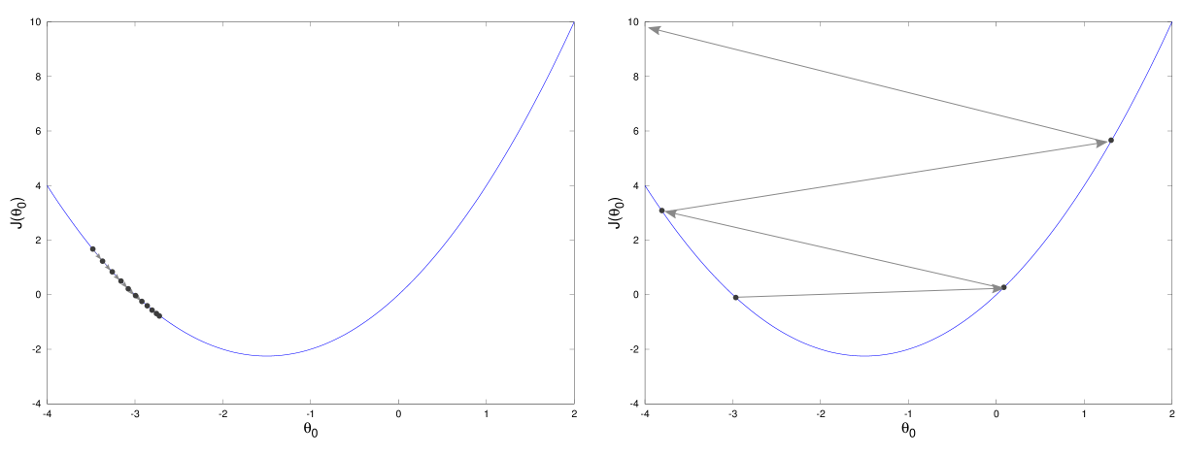
\includegraphics[width=\linewidth]{gradient_step_size}
\end{center}

If $\alpha_k$ is chosen with the \textbf{backtracking procedure} (Armijo rule) then the
algorithm converges to a stationary point of $f$. The idea is to start from
an initial value for $\alpha_k$, and then reducing it as
$\alpha_k=\phi\alpha_k$ with $\phi<1$ until the following condition is met:
$$f(x_k-\alpha_k\nabla f(x_k))\leq f(x_k)-\sigma\alpha_k \lVert \nabla
f(x_k)\rVert^2$$
where $\sigma$ is typically 0.25 and lies in the range $(0,0.5)$. The typical value
of $\phi$ is also 0.5.

Since we cannot run infinite iterations (there exists a truncation error), a
\textbf{stopping criteria} is needed:
\begin{itemize}
    \item We can use the property of $x^*$, where $\nabla f(x^*)=0$, to test
        whether the approximation $x_k$ is close to the solution within a
        specified tolerance. The criteria can be:
        \begin{itemize}
            \item \textbf{Absolute criterion}: $\lVert \nabla
                f(x_k)\rVert<\tau_A$
            \item \textbf{Relative criterion}: $\frac{\lVert \nabla
                f(x_k)\rVert}{\lVert \nabla f(x_0)\rVert}<\tau_R$
        \end{itemize}
    \item We can set a maximum number, $k^*$, of iterations.
    \item Additionally, as an heuristic, we stop when the norm of the gradient
        starts to flatten.
\end{itemize}
\begin{verbatim}
   input: f, x_0
   while stopping criteria holds:
        p_k = - grad(f(x_k))
        a_k = backtrack_procedure
        x_k = x_k + a_k * p_k
        k = k + 1
     output: x_k
\end{verbatim}
\paragraph{Initialization.} The initial point $x_0$ influences the
local minimum that is found. It is usually chosen randomly within the range of
$[-1,1]$ or $[0,1]$. Moreover, if $f(x)$ is convex, then every stationary
point is a global minimum of $f(x)$ and the choice of $x_0$ isn't important.
Otherwise when $f(x)$ isn't convex, we have to choose an initial point as
closest as possible to the \textit{right} stationary point.

\mbox{}

The algorithm introduced doesn't always work well because of the following
reasons:
\begin{itemize}
    \item If the objective function has flat areas or potholes on its loss
        surface, the procedure might be too slow or lead to a poor solution.
        Techniques such momentum, that inherit the rate of descent from
        previous steps, are often able to navigate through local potholes and flat
        regions. The idea is akin a stone rolling down a hill, gathering
        speed as it rolls down.
    \item If the components of the gradient have very different magnitudes,
        this causes problems for gradient-descent methods. 
    \item If the objective function has a steep region in its loss surface, the
        descent direction within this area changes quickly. This rapid change
        increase the likelihood of the divergence.
    \item The objective function may present non-differentiable points,
        which can create problems in calculating the gradient.
\end{itemize}

\subsection{Convex functions}

A convex set is a set where, for any two points within the set, the line
segment connecting these two points entirely lies within the set.

\begin{center}
    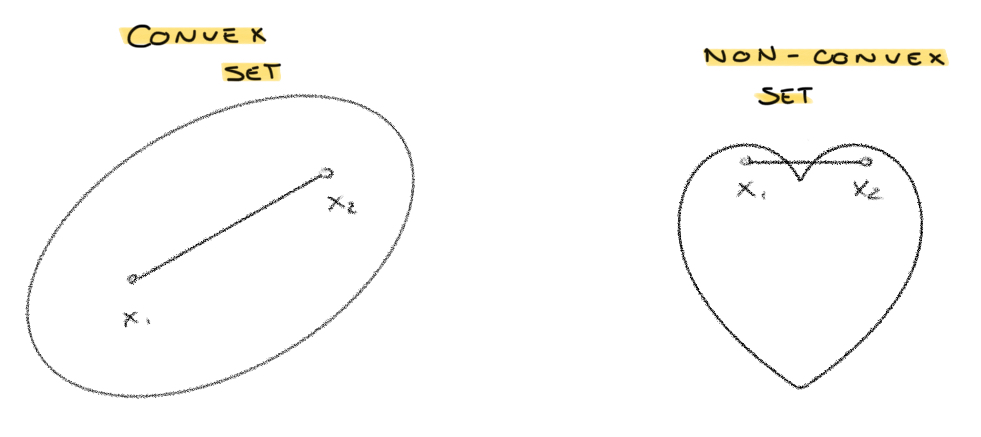
\includegraphics[width=0.65\linewidth]{convex_set}
\end{center}

\begin{definition}
    Let $f:\Omega\subset \mathbb{R}^n\to \mathbb{R}$, where $\Omega$ is a
    convex set. The function $f$ is (strictly) \textbf{convex} if, $\forall x,y\in\Omega$
    and $\forall\theta:0\leq\theta\leq1$, the following inequality holds:
    $$f(\theta x+(1-\theta)y) (<) \leq\theta f(x)+(1-\theta)f(y)$$
\end{definition}
In other words, the function of a point lying on the segment connecting $x$
and $y$ is below the segment connecting $f(x)$ and $f(y)$.
\begin{center}
    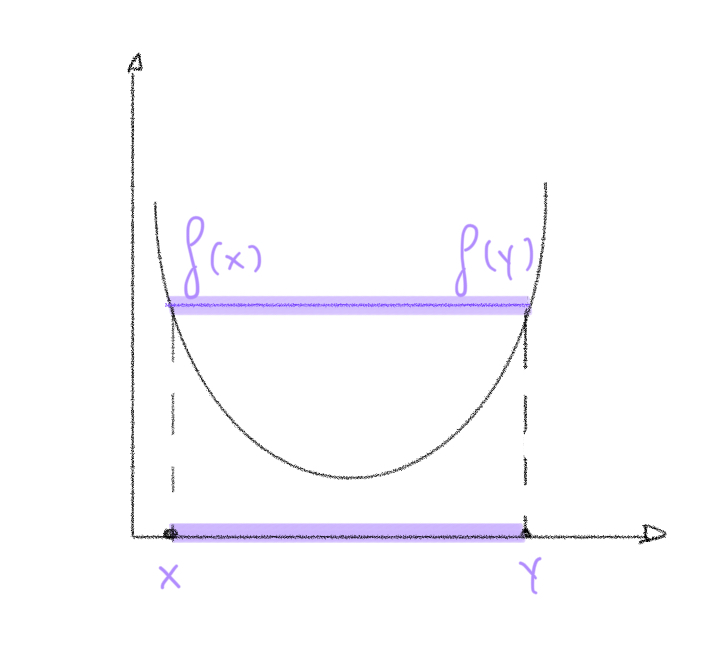
\includegraphics[width=0.5\linewidth]{convex_function}
\end{center}
\subsubsection{Quadratic functions}
An example of a strictly convex function is the quadratic function, which take the
following form:
$$f(x)=\frac{1}{2}x^TBx+c^Tx+(w)$$
with $b,c\in \mathbb{R}^n$ and $A\in \mathbb{R}^{n\times n}$ symmetric
positive definitive.

A typical quadratic function is the least square:
$$\lVert Ax-b\rVert^2$$
\begin{proof}
    \begin{equation*}
        \begin{aligned}
            \frac{1}{2}\lVert Ax-b\rVert^2 &=\frac{1}{2}(Ax-b)^T(Ax-b)\\ 
                                &=\frac{1}{2}(x^TA^T-b^T)(Ax-b)\\
                                &=\frac{1}{2}(x^TA^TAx-b^TAx-x^TA^Tb+b^Tb)\\ 
                                &=\frac{1}{2}x^T\underbrace{A^TA}_{\color{blue}B}x\underbrace{-b^TA}_{\color{blue}c^T}x+\frac{1}{2}b^Tb
        \end{aligned}
    \end{equation*}
    which is exactly the same as the above form.
\end{proof}
\subsubsection{Properties}
\begin{enumerate}
    \item If $f$ is convex, any point of local minimum is also a global
        minimum. 
    \item While a convex function can have multiple local minima, a strictly
        convex function has only \underline{one} local minimum, which is also
        a global minimum.
        \begin{center}
            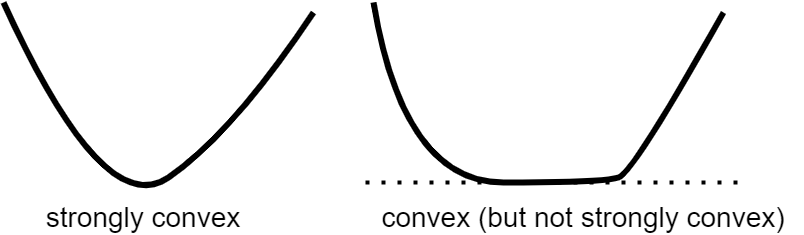
\includegraphics[width=0.75\linewidth]{strictly_convex}
        \end{center}
    \item If $f$ is convex and \underline{differentiable} any stationary point
        is a global minimum for $f$.
\end{enumerate}
\subsection{Variants of gradient descent algorithm}
\begin{itemize}
    \item Gradient descent with \textbf{momentum} method improves the
        convergence of the gradient descent method by memorizing and
        utilizing, at each step, what happened in the previous iteration. In
        particular:
        $$x_{k+1}=x_k-\alpha_k\nabla f(x_k)+\beta\Delta x_k$$
        where $\beta\in[0,1]$ and $\Delta x_k=x_k-x_{k-1}$ is the update
        obtained at iteration $k$.
        This update smooths the gradient updates and, thus, reduces the
        oscillations. This approach is analogous to a heavy ball in motion,
        where the momentum term represents the ball's resistance to change
        directions.
        \begin{center}
            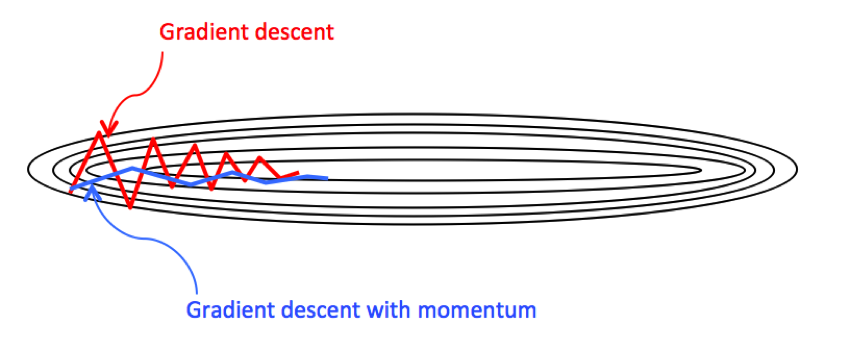
\includegraphics[width=0.75\linewidth]{gradient_momentum}
        \end{center}
    \item In machine learning, we typically train models by finding the
        optimal vector of parameters, denoted as $\theta$, that minimize a
        loss function $L(\theta)$. We can see this loss functions as the
        aggregate of individual losses $L_n$ incurred by each of the $N$ data
        points in the training set. Thus, the loss function is expressed as:
        $$L(\theta)=\sum_{n=1}^NL_n(\theta)$$
        The gradient of such loss function is then computed as follows:
        $$\nabla(\theta)=\sum_{n=1}^N\nabla L_n(\theta_k)$$
        In gradient descent, the optimization is performed by using
        the full training set and by updating the vectors of parameters
        according to:
        $$\theta_{k+1}=\theta_k-\alpha_k\sum_{n=1}^N(\nabla L_n(\theta_k))$$
        Evaluating the sum gradient may require expensive evaluations of the
        gradients from all individual functions $L_n$. If we consider the term
        $\sum_{n=1}^N(\nabla L_N(\theta_k))$, we can reduce the amount of the
        computation by taking a sum over a \underline{smaller set} of $L_n$.
        \begin{itemize}
            \item \textit{batch} $\to$ \underline{all} $L_n$ functions;
            \item \textit{mini-batch} $\to$ randomly choose a
                \underline{subset} of $L_n$
                functions. This can be a single $L_n$ or more. Large
                mini-batches lead to more stable convergence, but the
                calculations will be more expensive. Small mini-batches are
                quick to estimate, and the noise in gradient estimation might
                help to escape from some bad local optima.
        \end{itemize}
        The technique is used by \textbf{stochastic gradient descent}. It
        requires more iterations to converge, but with a small enough
        $\alpha_k$, it almost surely converges to a local minimum. Why use it?
        If there are constraints, such as memory limitations.

        Moreover, with stochastic gradient descent, we speak about \textbf{epoch} and not
        iterations. An epoch refers to the iterations necessary to ``see" all
        the data.
        \begin{equation*}
            \begin{aligned}
                \nabla L(\theta)&=\nabla L_{n_1}(\theta)\quad i=1,\
                n_1\in\{1\dots N\}\\
                \nabla L(\theta)&=\nabla L_{n_2}(\theta)\quad i=1,\ n_2\in\{1\dots
                N\}\setminus\{n_1\}\\
                \nabla L(\theta)&=\ldots
            \end{aligned}
        \end{equation*}
        The mini-batches do not repeat themselves before the entire epoch has
        been completed.
\end{itemize}
\cleardoublepage
\section{Probability and Statistics}
Probability focuses on modeling processes using random variables to capture
uncertainty. In contrast, statistics involves analyzing the observed data to
deduce the underlying processes that explain those observations.
\begin{definition}[State space $\Omega$]
    Set of all the possible results of a random experiment.
\end{definition}
\begin{example}
   Two coins 
   $$\Omega=\{TT,HT,TH,HH\}$$
\end{example}
\begin{definition}[Event space $\mathcal{A}$]
    A collection of results and $\mathcal{A}\subset\Omega$.
\end{definition}
\begin{definition}[Probability P]
    The probability of an event $\mathcal{A}$ is a function
    $P:A\to[0,1]\in
    \mathbb{R}$ that associates at each event $A$ a number called probability
    of $\mathcal{A}$.
    $$P(A)=\frac{\#(A)}{\#(\Omega)}$$
\end{definition}
\begin{example}
    $A\subset\Omega=\{TH,HT\}$
    $$P(A)=\frac{2}{4}$$
\end{example}
\begin{definition}[Conditional probability]
    The conditional probability of an event $B$ given the event $A$ is defined
    as:
    $$P(B|A)=\frac{P(A\cap B)}{P(A)}$$
    with $P(A)>0$.
\end{definition}
\begin{example}
    $A=\{\text{The first card is of seed heart}\}$ \\
    $B=\{\text{The second card is of seed heart}\}$
    $$
    \begin{aligned}
        P(A)&=\frac{13}{52}=\frac{1}{4}\\
        P(B|A)&=\frac{12}{51}
    \end{aligned}
    $$
    $A$ and $B$ are events dependent.
\end{example}
\begin{example}
   Toss a coin three times\\
   $\Omega=\{TTT,TTH,THT,HTT,HHT,HTH,THH,HHH\}$\\ 
   $A=\{\text{two }T\}$
   $B=\{\text{one } H\text{ and one }T\}$\\
   $P(A)=\frac{4}{8}\quad P(B)=\frac{6}{8}=\frac{3}{4}$\\
   $A\cap B=\{TTH,THT,HTT\}$
   $$P(A|B)=\frac{\frac{3}{8}}{\frac{3}{4}}=\frac{3}{8}\frac{4}{3}=\frac{1}{2}$$
   $$P(B|A)=\frac{\frac{3}{8}}{\frac{1}{2}}=\frac{3}{4}$$
\end{example}
\begin{definition}
    Two events $A$ and $B$ are \underline{independent events} if and only if:
    $$P(A\cap B)=P(A)\cdot P(B)$$
    and that means
    $$P(A|B)=P(A)\quad P(B|A)=P(B)$$
    That can be extended to multiple events. In fact, if
    $$P(A_1\cap A_2\ldots \cap A_n)=\prod_{i=1}^nP(A_i)$$
    then $A_1,A_2\ldots A_n$ are independent events.
\end{definition}
\subsection{Random variables}
\begin{definition}[Random variable]
    A random variable is a function $X:\Omega\to \mathbb{R}$ which associates
    each result $\omega\in\Omega$ to a number $x\in \mathbb{R}$.
\end{definition}
\begin{definition}
    We refer to $\mathcal{T}$ as the \textbf{target space of $X$} or
    \textbf{support of $X$} that is the set of all possible values of a random
    variable $X$.
    $$\{x|x=X(\omega),\quad\omega\in \mathbb{R}\}$$
\end{definition}
A random variable is:
\begin{itemize}
    \item \textbf{Discrete} if $\mathcal{T}$ is constituted by a
        \underline{countable} set of elements.
    \item \textbf{Continue} if $\mathcal{T}$ is an interval or an union of
       intervals of \underline{real} numbers. 
\end{itemize}
\clearpage
\begin{example}
   Toss a coin twice\\ 
   $\Omega=\{TT,TH,HT,HH\}$\\
   $X\underset{\omega\in\Omega}{(\omega)}=\{\text{number of }H\}$\\
   $X(TT)=0\ X(TH)=1,\ X(HT)=1,\ X(HH)=2$
   $$\mathcal{T}=\{0,1,2\}$$
   $X$ is discrete r.v.
\end{example}
\begin{example}
   Roll a die more times until we get 6\\ 
   $\Omega=\{n_1,n_2\ldots6\}$ $n_i=\{1,\ldots5\}$\\ 
   $Y=\{\text{number of rolls before getting 6}\}$ 
   $$T=\{1,2,3,4\ldots\}$$
   $Y$ is discrete r.v. because it has the same cardinality as integers.
\end{example}
\begin{example}
   A client enters a bank\\ 
   $Z=\{\text{time before the arrival of the client}\}$
   $$\mathcal{T}=[a,b]\subset(0,\infty)$$
   $Z$ is continuous r.v.
\end{example}
Now we will consider particular functions that describe the behavior of random
variables, specifically the values that can be obtained from random variables.
\subsubsection{Discrete random variables}
\begin{definition}[Probability mass function]
    The \textbf{probability mass function (PMF)} represents the probability that a
    random variable $X$ takes on a specific value $x$. Mathematically, this
    can be expressed as: 
    $$f_x:\mathcal{T}_x\to[0,1]$$
    $$\forall x\in \mathcal{T}_x,f_x(x)=P(X=x)$$
\end{definition}
In other words, it represents the probability distribution of a discrete
random variable has over its target space.
\begin{example}
   $\Omega=\{TT,TH,HT,HH\}$\\
   $X=\{\text{number of }H\}$\\
   $\mathcal{T}_x=\{0,1,2\}$\\
   $f_x:\{0,1,2\}\to[0,1]$
   $$
   \begin{aligned}
       f_x(0)&=P(X=0)=\frac{1}{4}\\
       f_x(1)&=P(X=1)=\frac{2}{4}=\frac{1}{2}\\
       f_x(2)&=P(X=2)=\frac{1}{4}
   \end{aligned}
   $$
   This shows that the r.v. has most often the value 1.
   \begin{center}
       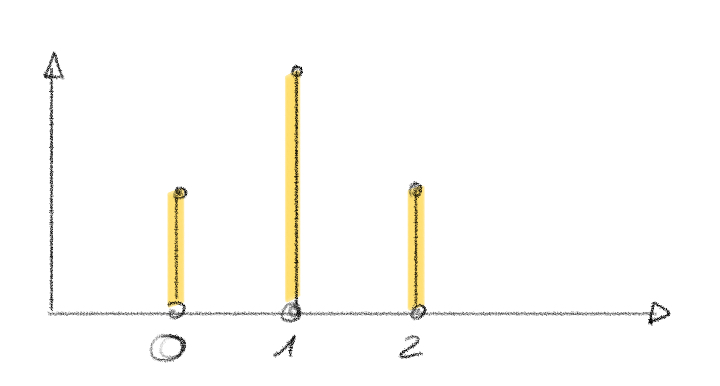
\includegraphics[width=0.5\linewidth]{pmf}
   \end{center}    
\end{example}
Moreover, the PMF has these properties:
\begin{enumerate}
    \item $f_x(x)\geq0\quad\forall x\in\mathcal{T}_x$
    \item $\sum_{x\in\mathcal{T}_x}f_x(x)=1$
    \item $A\subset\Omega,P(X=x\in A)=\sum_{x\in A}f_x(x)$
\end{enumerate}
Some examples of PMF are:
\begin{itemize}
    \item \textbf{Uniform distribution}: the r.v takes on all possible values
        in its target space with equal probability. 
        $$f_x(x)=\frac{1}{N}$$
        where $N=\#(\mathcal{T}_x)$.
    \item \textbf{Poisson distribution}: is used to model rare events and it
        describe the number of events happening in a given unit of time.
        $$f_x(x)=e^{-\lambda}\frac{-\lambda}{x!}$$
        where $\lambda$ is the mean and the standard deviation.
\end{itemize}
\subsubsection{Continuous random variables}
\begin{definition}[Probability density function]
    $X$ is a continuous r.v. if 
    $$f_x:\mathcal{T}_x\to \mathbb{R}$$
    $$P(a\leq X\leq b)=\int_a^b f_x(x)dx$$
    where $[a,b]$ is an interval in $\mathbb{R}$.
\end{definition}
In contrast to discrete r.v., the probability of a continuous r.v. taking a
particular value is \underline{zero}. In fact:
$$\text{If }a=b\implies\int_a^af_x(x)dx=0$$
In other words, the PDF represents the probability of the r.v. falling
\textsc{within a particular range of values}, as opposed to taking on any
one value.
\begin{center}
    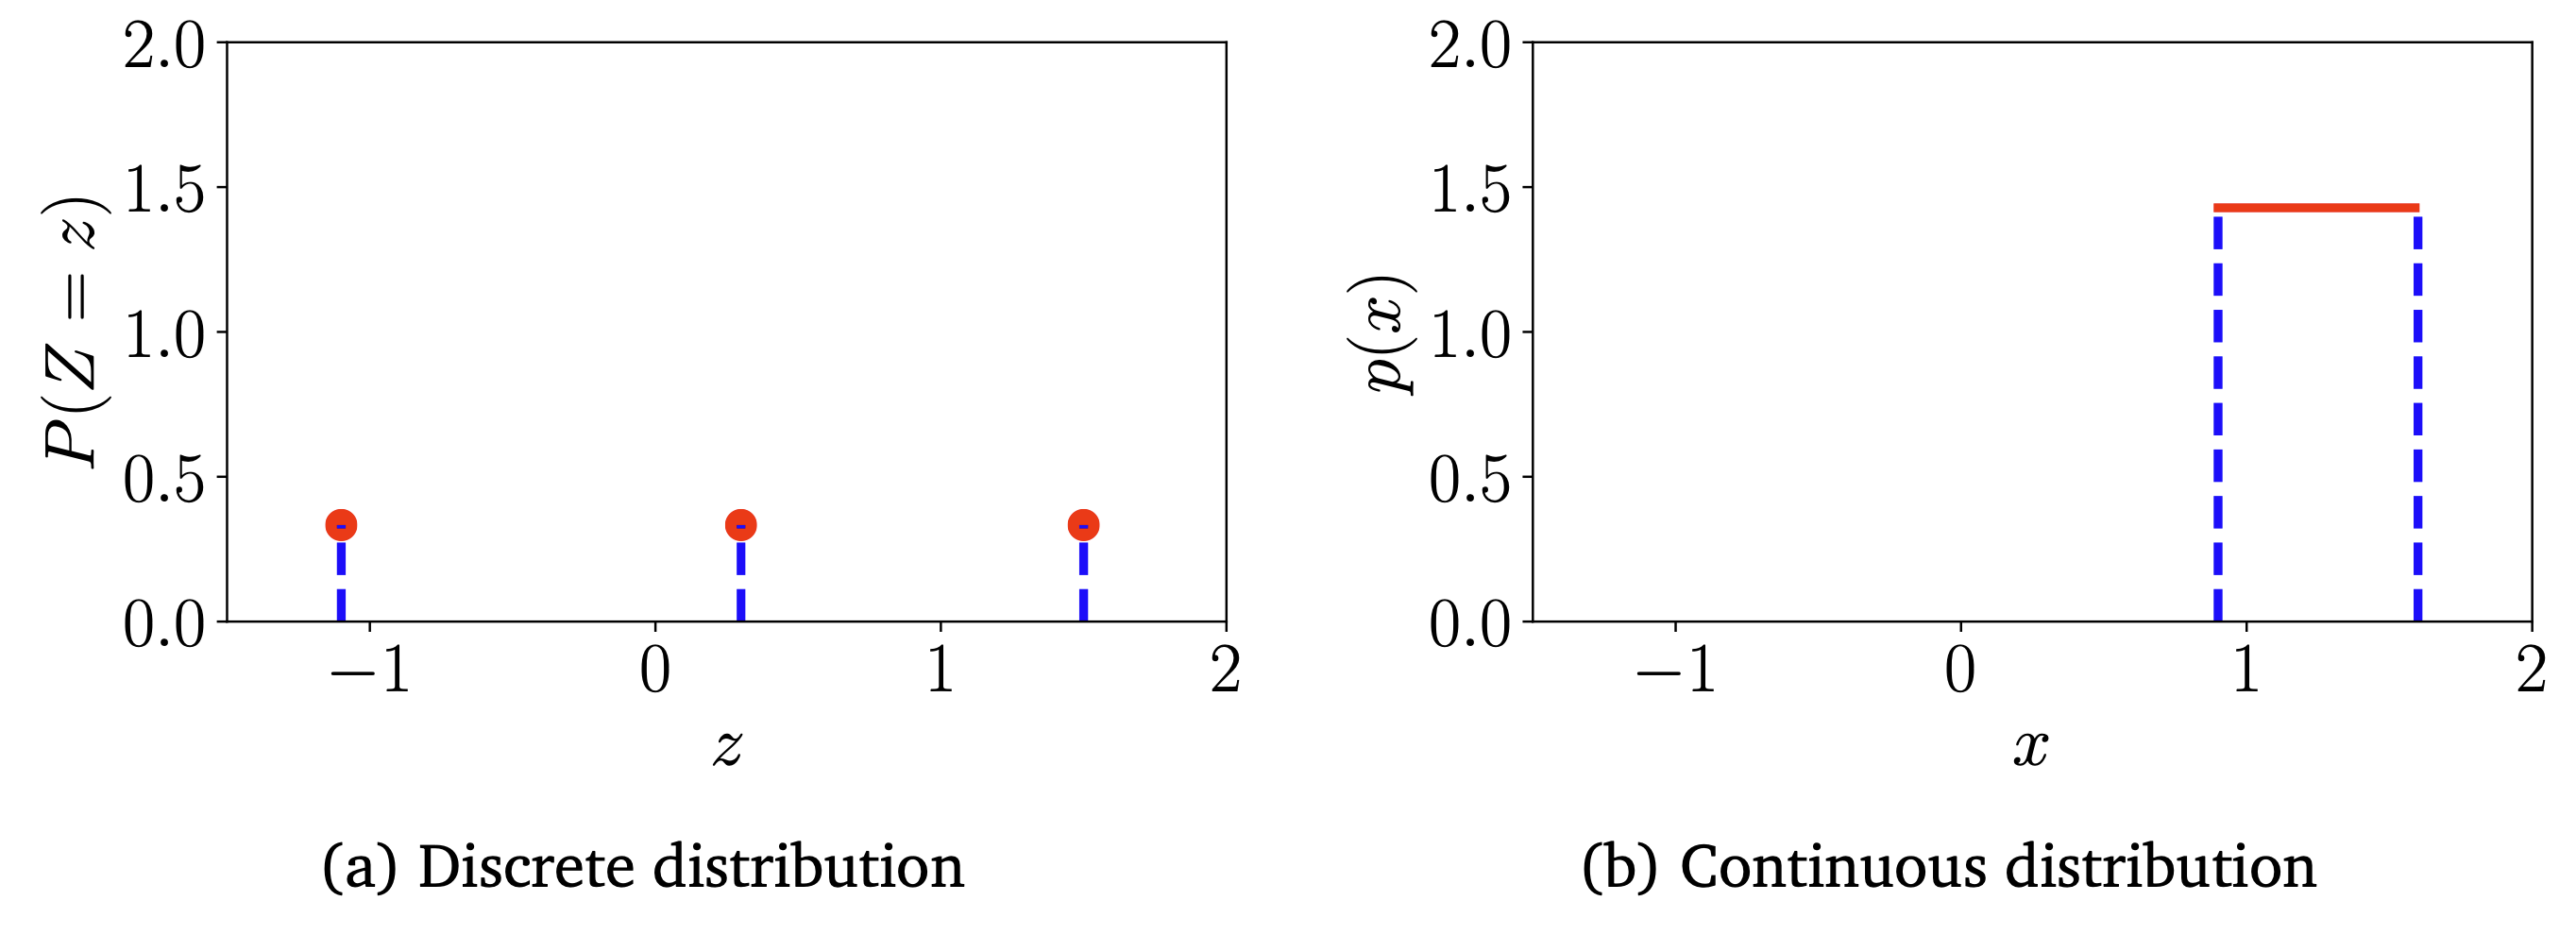
\includegraphics[width=\linewidth]{pmf_vs_pdf}
\end{center}
Moreover, the PDF has these properties:
\begin{enumerate}
    \item $f_x(x)\geq0\quad\forall x\in\mathcal{T}_x$
    \item $\int_a^bf_x(x)dx=1$
\end{enumerate}
\begin{example}
    $X$ continuous r.v.\\ 
    $f_x(x)=3x^2\quad0\leq x\leq 1\quad T_x=[0,1]$\\ 
    $P(X\in[0.2,0.6])=P(0.2\leq X\leq 0.6)?$
    $$
    \begin{aligned}
        P(0.2\leq X\leq
        0.6)&=\int_{0.2}^{0.6}3x^2dx=x^3|_{x=0.2}^{0.6}=(0.6^3-0.2^3)=0.208\\
    \end{aligned}
    $$
\end{example}
Some examples of PDF are:
\begin{itemize}
    \item \textbf{Uniform distribution}
        $$f_x(x)=\frac{1}{b-a}\quad x\in[a,b]=\mathcal{T}_x$$
    \item \textbf{Normal distribution (Gaussian)}
        $$f_x(x)=\frac{1}{\sigma\sqrt{2\pi}}e^{\frac{-(x-\mu)^2}{2\sigma^2}}\quad
        x\in \mathbb{R}$$
        where $\mu,\sigma$ are respectively the mean and the standard deviation.
        \begin{center}
            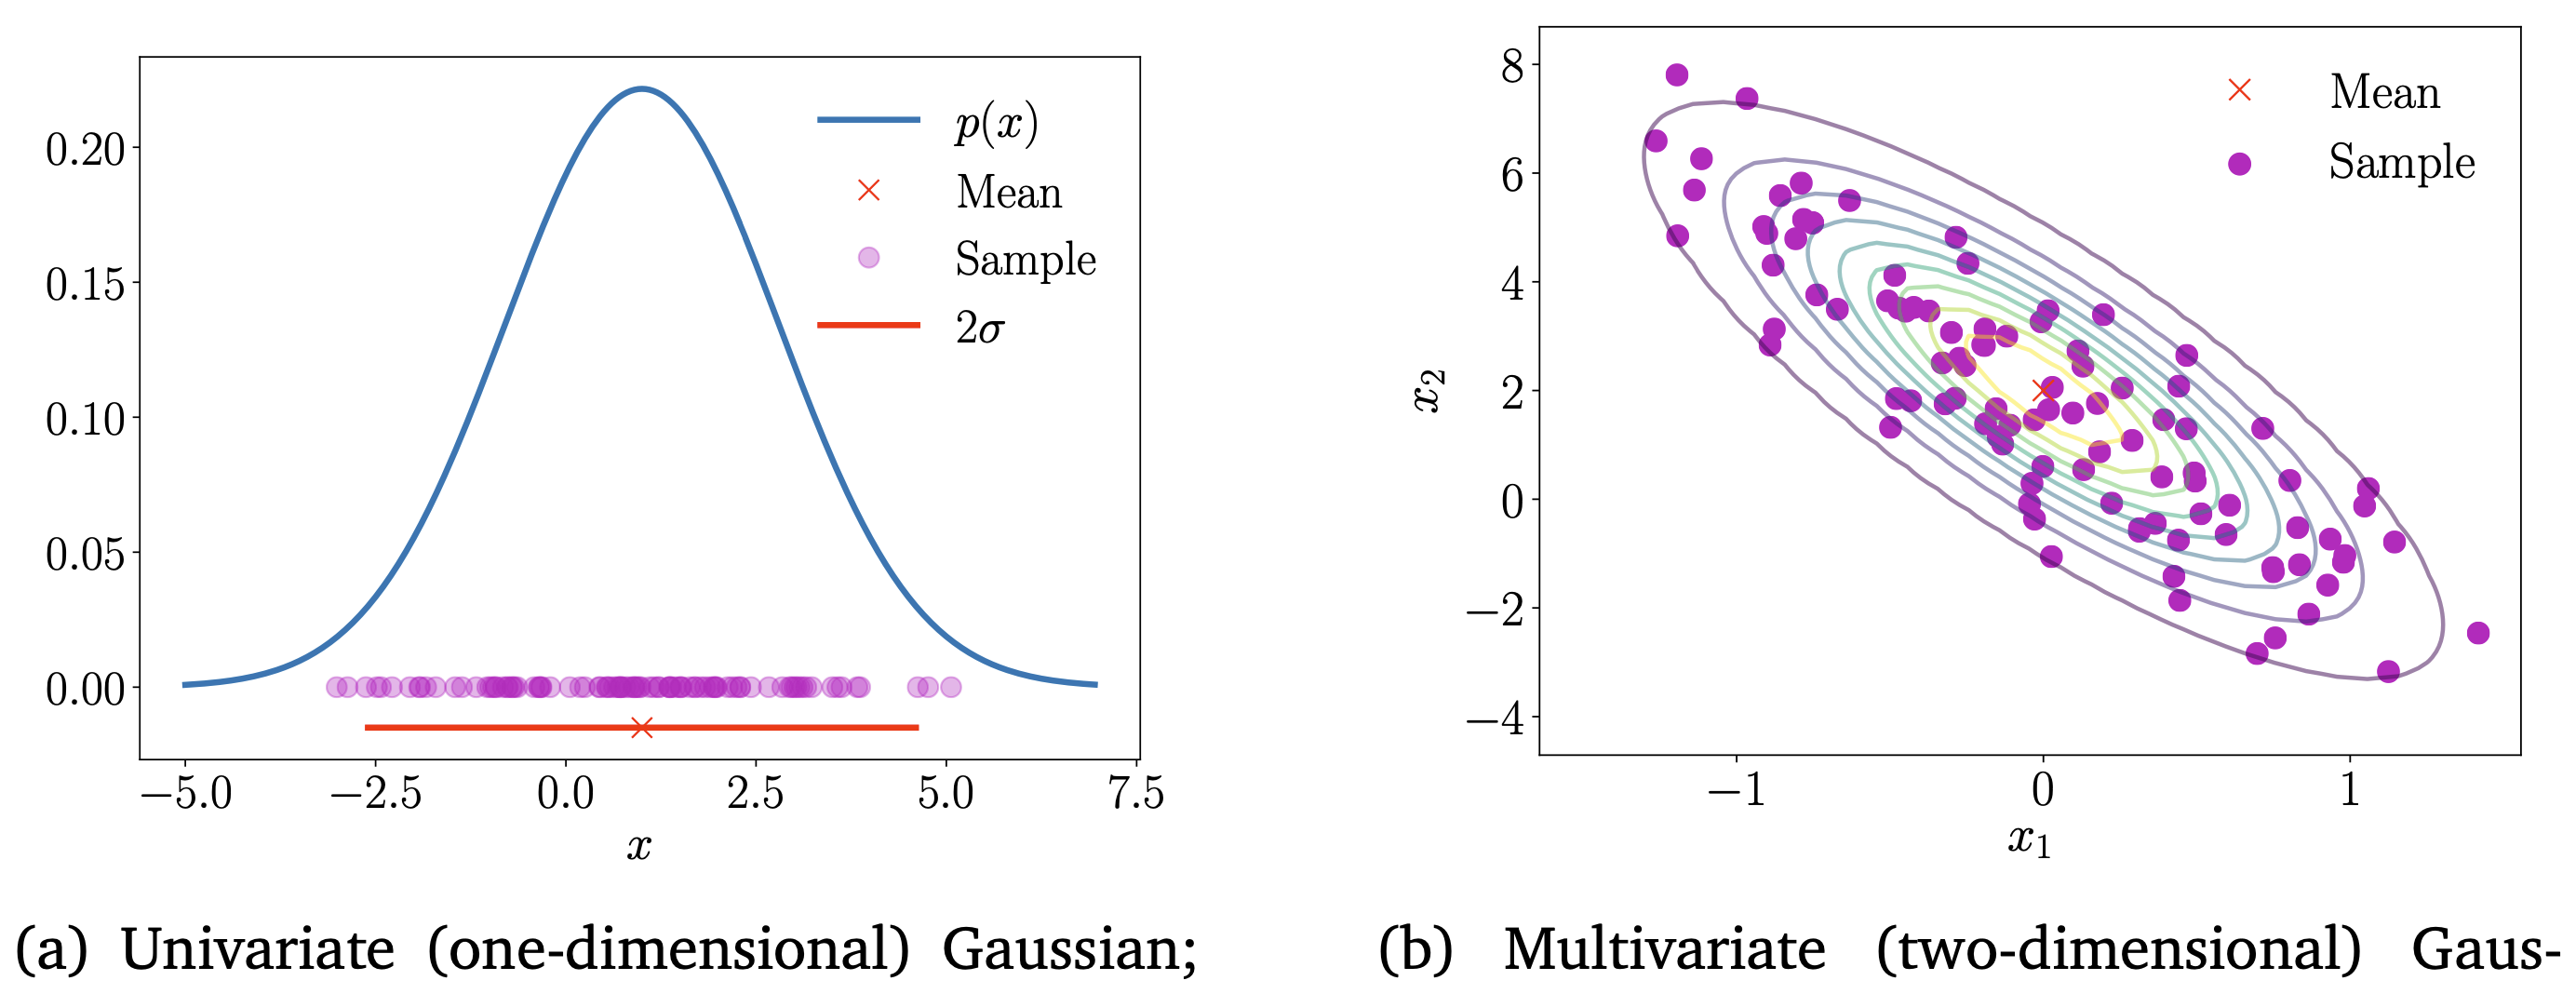
\includegraphics[width=\linewidth]{gaussian}
        \end{center}
        The special case of the gaussian with $\mu=0\text{ and }\sigma=1$ is
        referred as \textit{standard normal distribution}.
\end{itemize}
\subsection{Multiple random variables}
\begin{definition}
    \textbf{Univariate} refers to the distribution of a single r.v., while
    \textbf{multivariate} refers to the distributions of more than one r.v.
\end{definition}
\paragraph{Multivariate Normal distribution.}
$$\mathcal{N}(x\ | \ \mu, \Sigma)=(2\pi)^{-\frac{D}{2}}\left\lvert
\Sigma\right\rvert^{-\frac{1}{2}}e^{(x-\mu)^T\Sigma^{-1}(x-\mu)}$$
where $x=(x_1,\ldots,x_D)$. When the Gaussian distribution has $\mu=0$ and
$\Sigma=I$, it is referred to as \textit{standard normal distribution}.
\begin{definition}[Joint probability]
    The target space of each of the \textbf{joint probability} is the
    Cartesian product of the target spaces of each of the random variables.
    Mathematically, considering two random variables $X$ and $Y$ and their
    target spaces, $\mathcal{T}_X$ and $\mathcal{T}_Y$:
    $$\mathcal{T}_{XY}=\mathcal{T}_X\times \mathcal{T}_Y=\{(t_X,t_Y)\ |
    \ t_X\in\mathcal{T}_X,t_Y\in\mathcal{T}_Y\}$$
    The joint probability is defined as:
    $$f_{XY}:\mathcal{T}_{XY}\to[0,1]$$
    $$f_{XY}(x_i,y_j)=P(X=x_i,Y=y_j)=\frac{n_{ij}}{N}\quad x_i,y_j\in\mathcal{T}_{XY}$$
    where $n_{ij}$ is the number of the events with state $x_i$ and $y_j$ and
    $N$ the total number of the events.
    We can also say that the joint probability is the probability of the
    intersections of both events, such that $P(X=x_i,Y=y_j)=P(X=x_i\cap
    Y=y_j)$.
\end{definition}
\begin{center}
    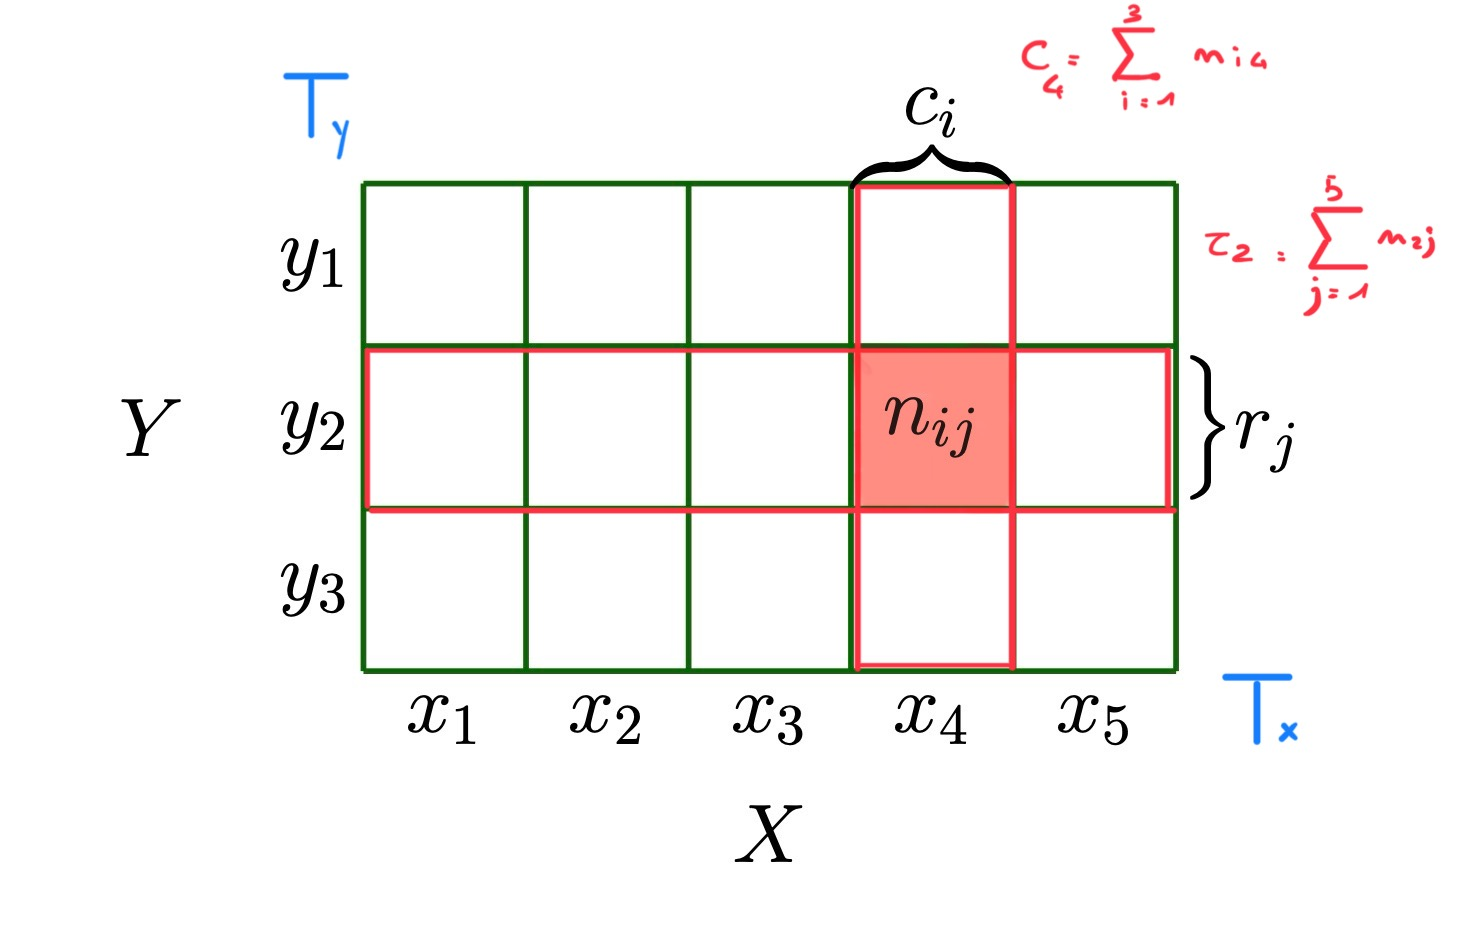
\includegraphics[width=0.65\linewidth]{marginal_probability}
\end{center}
\begin{definition}[Marginal probability] It's the probability of a single
    event occurring, independent of other event. This can be computed as the
    sum of the row or column: 
    $$
    \begin{aligned}
        f_X(x_i)=P(X=x_i)&=\frac{c_i}{N}\\
        f_Y(y_j)=P(Y=y_i)&=\frac{r_i}{N}
    \end{aligned}
    $$
    where $c_i$ and $r_i$ are respectively the $i$th column and $j$th row of the
    probability table.
\end{definition}
\begin{definition}[Conditional probability]
    It's the probability that an event occurs given that another specified
    event has \underline{already} happened. This can be computed using the
    following formulas: 
    $$
    \begin{aligned}
        P(Y=y_j\ |\ X=x_i)&=\frac{P(X=x_i\cap
        Y=y_j)}{P(X=x_i)}=\frac{n_{ij}}{c_i}\\
        P(X=x_i\ |\ Y=y_j)&=\frac{P(Y=y_i\cap X=x_j)}{P(Y=y_i)}=\frac{n_{ij}}{r_j}
    \end{aligned}
    $$
\end{definition}
Given the definitions of the marginal and conditional probability for ours
r.v. we can now present two rules in probability theory:
\begin{itemize}
    \item \textbf{Sum rule}:
        $$
        f_X(x_i)=\begin{cases}
            \sum_{y_j\in\mathcal{T}_y} f_{XY}(x_i,y_j) & \text{if }y\text{ is
            discrete} \\
                \int_{\mathcal{T}_Y}f_{XY}(x_i,y_j)dy_j & \text{if }y\text{ is
                continuous}
        \end{cases}
        $$
    \item \textbf{Product rule}: the joint distribution of two random
        variables can be factorized as conditional distribution and marginal
        distribution
        {\color{blue}$$f_{XY}(x_i,y_j)=P(Y=y_j\ |\ X=x_i)f_X(x_i)$$}
        or 
        {\color{blue}$$f_{XY}(x_i,y_j)=P(X=x_j\ |\ Y=y_i)f_Y(y_j)$$}
\end{itemize}
\begin{theorem}[Bayes's theorem]
    The bayes theorem states how to update the prior with new information
    given by the likelihood. In particular: 
    $$\underbrace{P(x\ |\
    y)}_{\text{posterior}}=\frac{\overbrace{P(y\ |\ x)}^{
    \text{likelihood}}\overbrace{P(x)}^{\text{prior}}}{\underbrace{P(y)}_{\text{evidence}}}$$

    \begin{itemize}
        \item \textbf{Prior}: encapsulates our subjective prior knowledge of
            the \underline{unobserved} variable $x$ before observing any data.
            We can choose any prior that makes sense.
        \item \textbf{Likelihood}: it is the probability of the data $y$ if we
            were to know the latent variable $x$.
        \item \textbf{Posterior}: what we are interest in, i.e, what we know
            about $x$ after having observed $y$.
        \item \textbf{Evidence}: acts like a normalizing constant. 
    \end{itemize}
\end{theorem}
It's possible to focus on some statistic of the posterior, such as the maximum
of the posterior.
$$\argmax_x{P(x\ |\ y)}\underset{\text{Bayes}}=\frac{P(y\ |\
x)P(x)}{\cancel{P(y)}}$$
\subsection{Summary statistics}
The statistic of a r.v. is a deterministic function of that r.v.. The summary
statistic provide one useful view of how a r.v. behave and provide
numbers that summarize and characterize it.

\begin{definition}[Expected Value]
    The expected value of a function $g:\mathbb{R}\to \mathbb{R}$ of a
    \underline{univariate} r.v. $X$ is given by
    $$\mathbb{E}_X[g(x)]=\begin{cases}
        \int_{\mathcal{T}_X}g(x)f_X(x) & \text{if }X\text{ is continuous}\\ 
        \sum_{x\in\mathcal{T}_X} g(x)f_X(x) & \text{if }X\text{ is discrete}
    \end{cases}$$
    For \underline{multivariate} r.v. $X=[X_1,\ldots,X_D]$, the
    expected value is a vector of expected values of the respective univariate
    r.v.: 
    $$
    \mathbb{E}_X[g(x)]=\begin{bmatrix}
        \mathbb{E}_{X_1}[g(x_1)]\\
        \vdots\\
        \mathbb{E}_{X_D}[g(x_D)]
    \end{bmatrix}\in \mathbb{R}^D
    $$
\end{definition}
The definition of the mean is a special case of the expected value, obtained
by choosing $g$ to be the identity function $g(x)=x$.
\begin{definition}[Mean]
    The mean of a multivariate r.v. $X=[X_1,\ldots,X_D]$ is an average and is
    defined as 
    $$
    \mathbb{E}_X[g(x)]=\begin{bmatrix}
        \mathbb{E}_{X_1}[x_1]\\
        \vdots\\
        \mathbb{E}_{X_D}[x_D]
    \end{bmatrix}\in \mathbb{R}^D
    $$
    where each one corresponds to 
    $$\begin{cases}
        \int_{\mathcal{T}_X}xf_X(x) & \text{if }X\text{ is continuous}\\ 
        \sum_{x\in\mathcal{T}_X} xf_X(x) & \text{if }X\text{ is discrete}
    \end{cases}$$
\end{definition}
The mean is also called the expected value because it represents the most
probable value.
\begin{example}
    $X$ continuous r.v.\\ 
    $f_x(x)=3x^2\quad0\leq x\leq1$\\ 
    mean of $f_x(x)$?
    $$
        \mathbb{E}_x[x]=\int_0^1xf_x(x)dx=\int_0^13x^3dx=\frac{3}{4}x^4\ |_{x=0}^1=\frac{3}{4}
    $$
\end{example}
\begin{definition}[Covariance]
    The Covariance between two univariate random variable $X,Y\in \mathbb{R}$
    is given by the expected product of their deviations from their respective
    means:
    $$\text{Cov}_{X,Y}[x,y]=\mathbb{E}_{X,Y}[(x-\mathbb{E}_X[x])(y-\mathbb{E}_Y[y])]$$
    When dealing with two multivariate r.v., $X=(X_1,\ldots,X_D)$ and
    $Y=(Y_1,\ldots,Y_E)$, the covariance between $X$ and $Y$ is defined as
    follows: 
    $$\text{Cov}_{X,Y}[x,y]=\begin{bmatrix}
        \text{Cov}[x_1,y_1] & \ldots &
        \text{Cov}[x_1,y_E] \\ 
        \vdots & \ddots & \vdots \\ 
        \text{Cov}[x_D,y_1] & \ldots & \text{Cov}[x_D,y_E]
    \end{bmatrix}\in \mathbb{R}^{D\times E}$$
    The $D\times E$ matrix is called the \textbf{cross-covariance matrix} of
    the two multivariate r.v. $X$ and $Y$.
\end{definition}
\begin{definition}[Variance]The covariance of a variable with itself $\text{Cov}_{X,X}[x,x]$ is called
    \textbf{variance} and is defined as follows:
    $$
        \begin{aligned}
            \mathbb{V}_X[x]&=\text{Cov}_X[x,x]\\
                           &=\begin{bmatrix}
                               \text{Cov}[x_1,x_1] & \ldots &
                               \text{Cov}[x_1,x_D] \\ 
                               \vdots & \ddots & \vdots \\ 
                               \text{Cov}[x_D,x_1] & \ldots & \text{Cov}[x_D,x_D]
                           \end{bmatrix}
        \end{aligned}
    $$
    The $D\times D$ matrix is called the \textbf{covariance matrix} of the
    multivariate r.v. $X$.
\end{definition}
The covariance indicates how two r.v. are related in terms of their
dimensions. However, since covariance lacks an upper bound, it doesn't provide
a clear indication how much they are related. To address this, a normalized
version of covariance, which constraints the range between -1 and 1, offer a
more convenient statistic to measure the relationship between two r.v.
\begin{definition}[Correlation]
    The correlation between two r.v. $X,Y$ is given by
    $$\text{corr}_{X,Y}[X,Y]=\frac{\text{Cov}_{X,Y}[x,y]}{\sqrt{\mathbb{V}_X[x]\mathbb{V}_Y[y]}}\in[-1,1]$$
\end{definition}
Positive correlation means that when $x$ grows, the $y$ is also expected to
grow. Negative correlation means that as $x$ increases then $y$ decreases
\begin{center}
    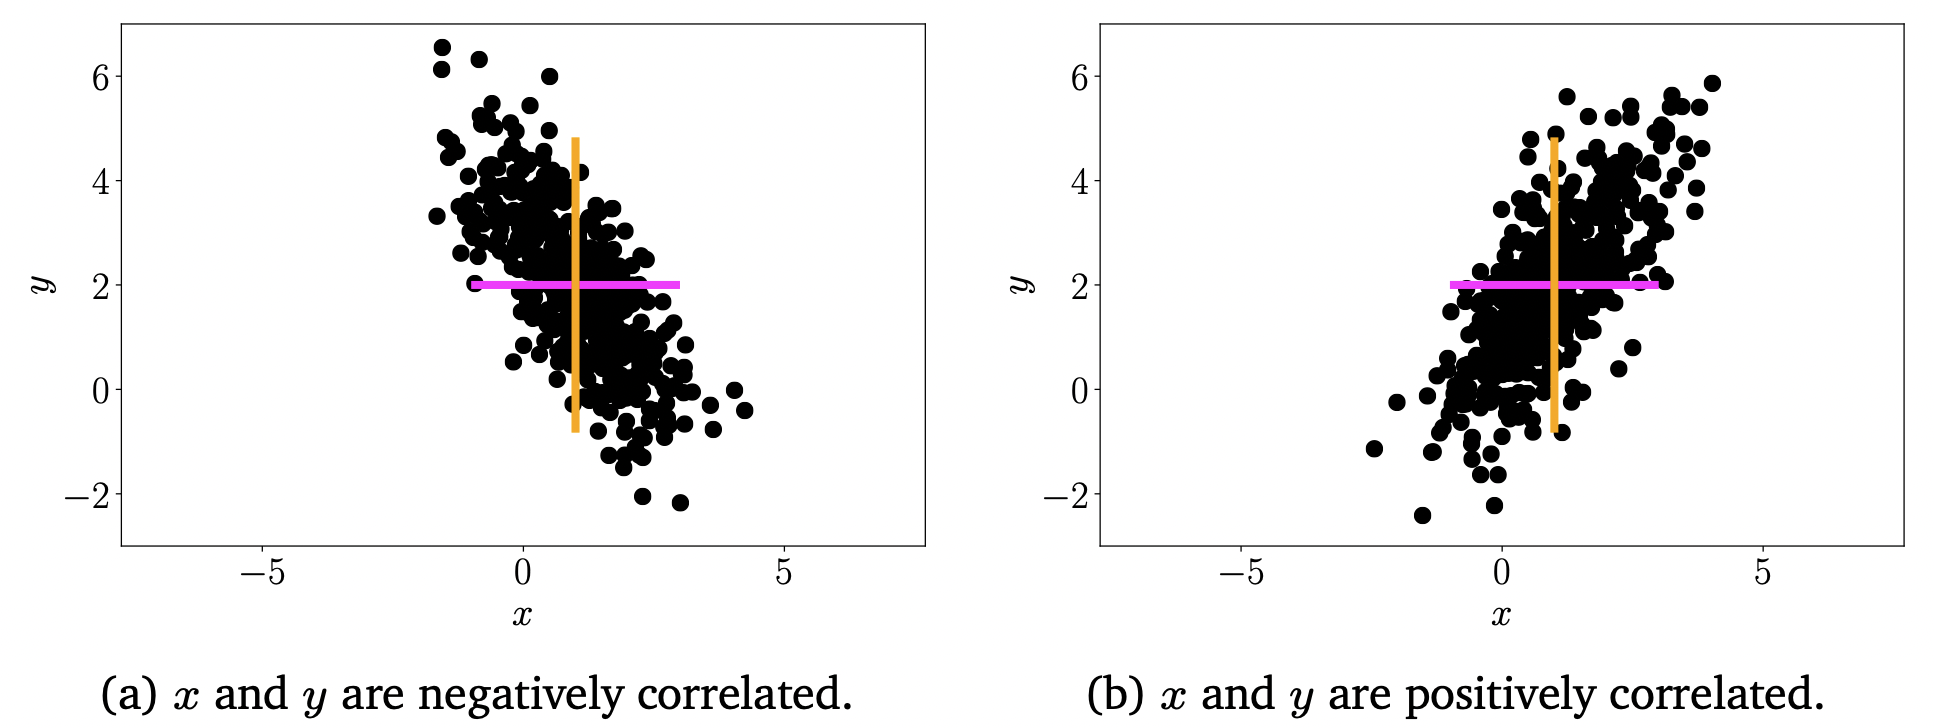
\includegraphics[width=\linewidth]{correlation}
\end{center}
\paragraph{Empirical statistics}
The definitions above are called population mean and population covariance, as
it refers to the true statistics for the population.
\begin{center}
    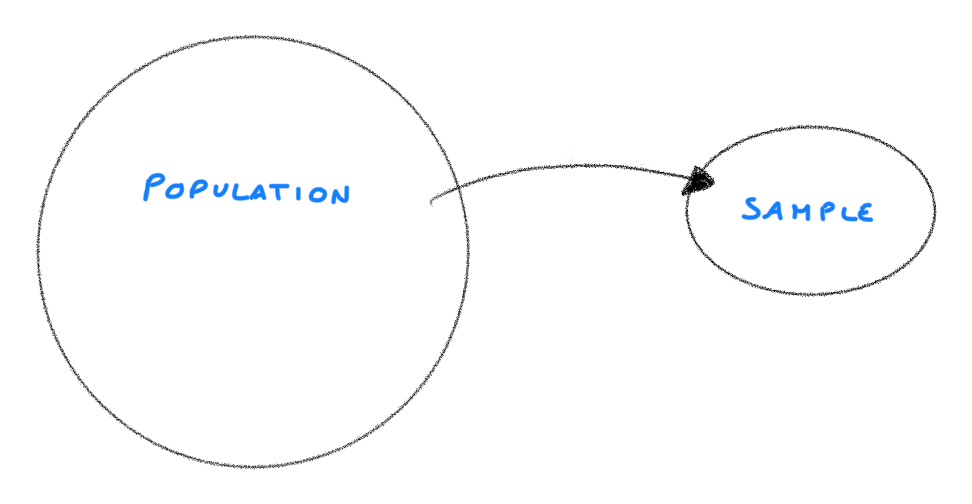
\includegraphics[width=0.5\linewidth]{population}
\end{center}
From a dataset that represents a sample of the population, we observe it and
infer some properties of the population:
\begin{itemize}
    \item \textbf{Empirical mean}:
        $$\bar{x}=\frac{1}{N}\displaystyle\sum_{i=1}^{N}x_i$$
    \item \textbf{Empirical variance}:
        $$\mathbb{V}_X[x]=\frac{1}{N}\displaystyle\sum_{i=1}^{N}(x_i-\bar{x})$$
    \item \textbf{Empirical standard definition}: 
        $$\sigma=\sqrt{\mathbb{V}_X[x]}$$
\end{itemize}
\subsection{Algebra of random variables}
Considering two r.v. $X=(X_1,\ldots,X_D)$ and $Y=(Y_1,\ldots,Y_D)$, then:
$$
\begin{aligned}
    \mathbb{E}_{X,Y}[x+y]&=\mathbb{E}_X[x]+\mathbb{E}_Y[y]\\
    \mathbb{E}_{X,Y}[x-y]&=\mathbb{E}_X[x]-\mathbb{E}_Y[y]\\
    \mathbb{V}_{X,Y}[x+y]&=\mathbb{V}_X[x]+\mathbb{V}_Y[y]+\text{Cov}_{X,Y}[x,y]+\text{Cov}_{Y,X}[y,x]\\
    \mathbb{V}_{X,Y}[x-y]&=\mathbb{V}_X[x]+\mathbb{V}_Y[y]-\text{Cov}_{X,Y}[x,y]-\text{Cov}_{Y,X}[y,x]\\
\end{aligned}
$$
\begin{definition}[Independence]
    Two r.v., $X$ and $Y$, are statistically independent if the joint
    probability of $X$ and $Y$ can be written as the product of their marginal
    probabilities:
    $$f_{X,Y}[x,y]=f_X[x]f_Y[y]$$
    Intuitively, this means that the two r.v. don't influence each other.
\end{definition}
If $X,Y$ are independent, then: 
$$
\begin{aligned}
    P(Y=y\ |\ X=x) &= P(Y=y)\\
    P(X=x\ |\ Y=y) &= P(X=x)\\
    \mathbb{V}_{X,Y}[x+y]&=\mathbb{V}_X[x]+\mathbb{V}_Y[y]\\
    \text{Cov}_{X,Y}[x,y] &= 0
\end{aligned}
$$
The viceversa of the last point doesn't hold.

\begin{definition}[Conditional Independence]
    Two r.v., $X$ and $Y$, are conditionally independent given $Z$ if and only
    if 
    $$P(X=x\cap Y=y\ |\ Z=z)=P(X=x\ |\ Z=z)P(Y=y\ |\ Z=z)$$
\end{definition}
\paragraph{Geometry.}r.v. can be considered vectors in a vector space of
probability distributions, and we can define inner product to obtain geometric
properties of it. Recall the definition of inner products
$\langle\cdot,\cdot\rangle:(x,y)\to \mathbb{R}$, so for zero mean r.v. $X$ and
$Y$
$$\langle X,Y\rangle=\text{Cov}_{X,Y}[x,y]\in \mathbb{R}^+$$
The \underline{length of a r.v. is the standard deviation}:
$$\lVert X\rVert=\sqrt{\text{Cov}_{X,Y}[x,x]}=\sqrt{\mathbb{V}[x]}=\sigma[x]$$
The longer the r.v, the more uncertain it is; and a r.v with length 0 is
deterministic.

We can interpret the \underline{angle $\theta$ between two r.v., $X$ and $Y$,
as their correlation}:
$$\cos\theta=\frac{\langle X,Y\rangle}{\lVert X\rVert \lVert
Y\rVert}=\frac{\text{Cov}_{X,Y}[x,y]}{\sqrt{\mathbb{V}_X[x]\mathbb{V}_Y[y]}}$$

Recall that two vectors are orthoganal if and only if:
$$X\perp Y\iff\langle X,Y\rangle=0$$
Therefore, they are orthogonal if and only if $\text{Cov}_{X,Y}[x,y]=0$.
\paragraph{Gaussian linearity.}
For two independent r.v., $X,Y$, we have:
$$
\begin{aligned}
    f_{X,Y}[x+y]&=\mathcal{N}(\mu_x+\mu_y,\Sigma_x+\Sigma_y) \\
    f_{X,Y}[\alpha x+\beta y]&=\mathcal{N}(\alpha\mu_x+\beta\mu_y,\alpha^2\Sigma_x+\beta^2\Sigma_y) 
\end{aligned}
$$
where $\alpha,\beta\in \mathbb{R}$. This means that in both cases, the result
will be a Gaussian distribution.
\cleardoublepage
\section{Machine Learning Problems}
In machine learning, our main goal, is to create models, or predictors,
that make good predictions on unseen data. The concept of a model can be seen
in two ways:
\begin{itemize}
    \item \textbf{as function (deterministic).} A predictor is a function:
        $$f:\mathbb{R}^D\to \mathbb{R}$$
        Here, the input vector $x$ is a $D$-dimensional (that has $D$
        features), and the function $f$, when applied to this vector, returns
        a real number. We will focus on linear functions, which can be
        represented as:
        $$f(x)=\theta^Tx$$
        where $\theta=[\theta_0,\theta_1,\ldots,\theta_D]$ and
        $x=[1,x^{(1)},\ldots,x^{(D)}]$ (we have concatenated an unit feature
        $x^{(0)}=1$ to $x$, which allows us to incorporate the bias term into
        the vector $\theta$).\\
        The parameters of the function are represented by $\theta$.
    \item \textbf{as multivariate probability distribution (probabilistic).}
        In this case, the parameters correspond to those of the distribution.
\end{itemize}
In order to obtain good predictions from a model, it's essential to adjust its
parameters using training data (learning). There are two main approaches to this
parameter adjustment: for non-probabilistic models, we use \textbf{empirical
risk minimization}, and for probabilistic models, we utilize the method of
\textbf{maximum likelihood} estimation.
\subsection{Empirical Risk Minimization}
\begin{center}
    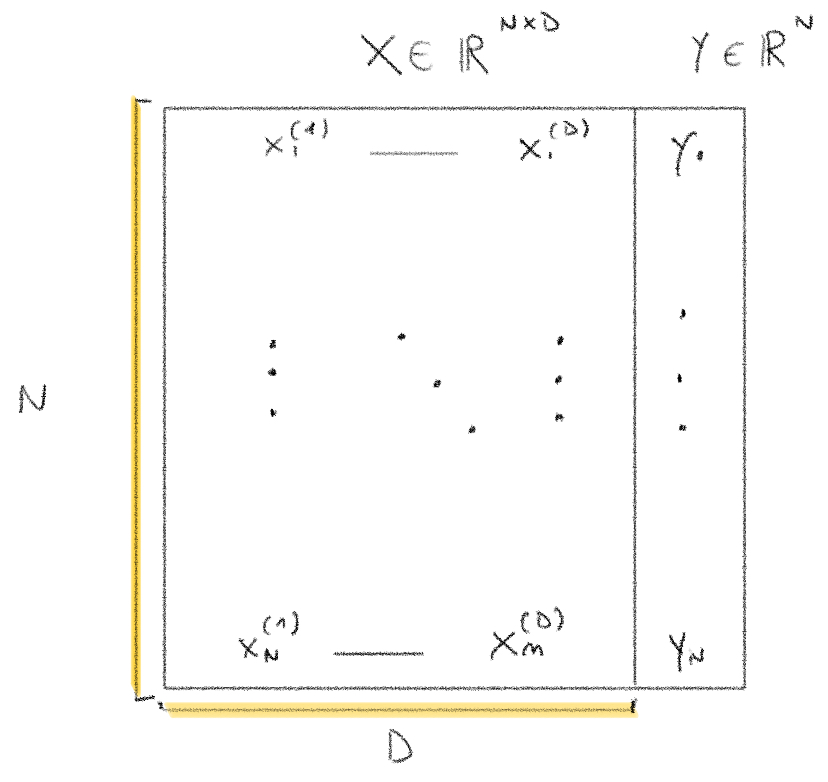
\includegraphics[width=0.5\linewidth]{dataset}
\end{center}
Given a dataset consisting of $N$ examples $x_n \in \mathbb{R}^D$ and
corresponding scalar labels $y_n \in \mathbb{R}$, we consider a supervised
learning scenario. In this setting, we work with pairs $(x_1, y_1), \ldots,
(x_N, y_N)$. The objective is to identify the optimal parameters $\theta^*$ of
a predictor $f(\cdot,\theta):\mathbb{R}^D\to \mathbb{R}$, such that the model
fits well the data. In other words, we aim for 
$$f(x_n,\theta^*)=\hat{y}\approx y_n\quad\forall n=1,\ldots,N$$
To define what it means to fit the data well, we need to specify a \textbf{loss
function} $\ell(y_n,\hat{y}_n)$, which take the ground truth label $y_n$ and
the prediction $\hat{y}_n$ as input and produces a non-negative number representing how
much error the model has been made on the particular prediction.

The optimal parameter vector $\theta^*$ is given by minimizing the average
loss of the set of $N$ training samples that is given by \textbf{empirical
risk}:
$$R_{\text{emp}(f,X,y)}=\frac{1}{N}\sum^{N}_{n=1}\ell(y_n,\hat{y}_n)$$
$$\theta^*=\min_{\theta\in\mathbb{R}^D}\frac{1}{N}\sum^{N}_{n=1}\ell(y_n,\hat{y}_n)$$
\begin{example}
    An example of a loss is the least-squares
    $\ell(y_n,\hat{y}_n)=(y_n-\hat{y}_n)$, thus:
    $$\theta^*=\min_{\theta\in\mathbb{R}^D}\frac{1}{N}\sum^{N}_{n=1}(y_n-f(x_n,\theta))^2$$
    where we substituted the predictor $\hat{y}_n=f(x_n,\theta)$. By using the
    linear predictor $f(x_n\theta)=\theta^Tx_n$ we obtain:
    $$\theta^*=\min_{\theta\in\mathbb{R}^D}\frac{1}{N}\sum^{N}_{n=1}(y_n-\theta^Tx_n)^2$$
    That is equivalently expressed in matrix form: 
    $$\theta^*=\min_{\theta\in\mathbb{R}^D}\frac{1}{N}\lVert y-X\theta\rVert^2$$
    This is known as the \textit{least-squares problem}.
\end{example}
However, we aren't interested in a predictor that only perform well on the
training data. Instead, we seek a predictor that performs well on unseen data
, i.e. the predictor generalizes well.
\begin{center}
    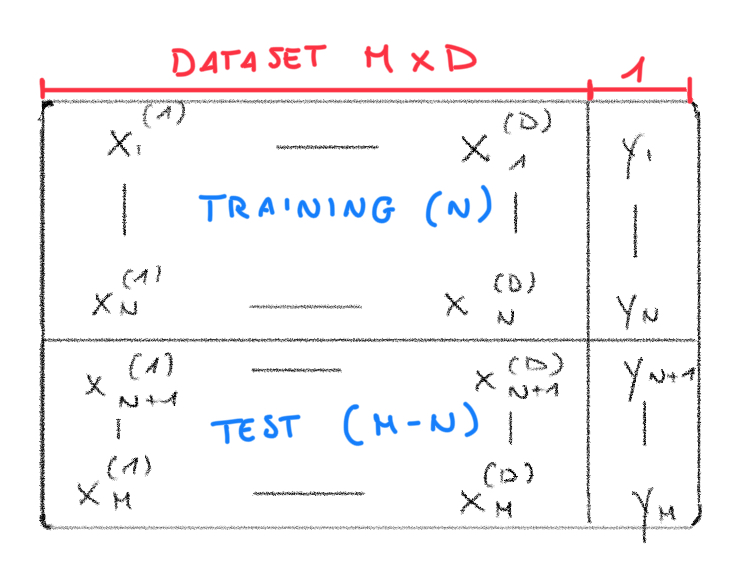
\includegraphics[width=0.5\linewidth]{dataset_traintest} 
\end{center}
Given a dataset constituted of $M$ examples $x_m\in \mathbb{R}^D$ and
corresponding scalar labels $y_m$, we divide the dataset into two parts: a
training set with $N$ examples and a \textbf{test set} with the remaining
$M-N$ examples. We simulate the unseen data by using this test set.

Now we are interested in finding a predictor $f$ (\underline{with parameters
fixed}) that minimized the \textbf{expected risk}:
$$R_{\text{true}}(f)=\mathbb{E}_{x,y}[\ell(y,f(x))]$$
Here, minimizing the expected risk means finding the predictor that has the
lowest loss when evaluated on the entire population, which in our scenario is
represented by the test set.
\paragraph{Regularization.}
When the test risk is much larger than the training risk, this is an
indication of \textbf{overfitting}, i.e. the predictor fits too closely to the
training data and doesn't generalize well to new data. This issue often arises
when utilizing overly complex models. To address this, we introduce a penalty
term involving $\theta$, which serves to reduce the model's complexity:
$$\theta^*=\min_{\theta\in\mathbb{R}^D}\frac{1}{N}\lVert
y-X\theta\rVert^2+\lambda \lVert \theta\rVert^2$$
The additional term $\lVert \theta\rVert^2$ is called \textit{regularizer},
and the hyperparameter $\lambda$ is the \textit{regularization parameter}.
This hyperparameter trades off minimizing the loss on the training set and the
magnitude of the parameter $\theta$. A sign of overfitting is when the values
of the parameters become large. By applying the penalty term, we essentially
restrict the vector $\theta$ to remain closer to the origin.
\begin{center}
    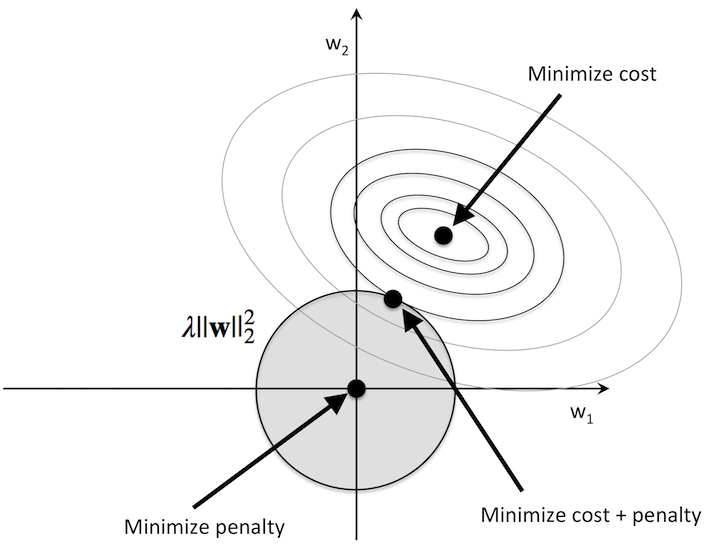
\includegraphics[width=0.75\linewidth]{regularization}
\end{center}
\subsection{Parameter estimation of a probability distribution}
In a supervise learning setting, we have a dataset consisting of $N$ pairs\\
$(x_1,y_1)\ldots,(y_N,y_N)$, where each $x_n\in \mathbb{R^D}$ and $y_n\in
\mathbb{R}$ (for $n=1,\ldots,N$). We assume these pairs are
\underline{independently identically distribuited}.

Each vector $x_n$ is drawn from an unknown probability distribution $x_n\sim
P(x)$. The corresponding label $y_n$ is considered as an output from a
conditional probability distribution of labels given the examples for the
particular parameter setting $\theta$, $y_n\sim P_\theta(y\ |\ x_n)$.
\subsubsection{Maximum Likelihood Estimation}
With this framework, learning a model can be thought as finding the parameters
of a distribution $P_\theta(y\ |\ x)$ (the likelihood) that maximized the
probability of observing $y$, given $x$. Therefore, we must solve the
optimization problem: 
$$\theta^*=\argmax_{\theta}P_\theta(y\ |\ x)$$
which is called \textbf{Maximum Likelihood Estimation (MLE)}, because the
parameters $\theta^*$ are chosen such that they maximize the likelihood.

Given the assumption of independence, we can factorized the whole dataset
into a product o the likelihoods of each individual example: 
$$P_\theta(x,y)=\prod_{n=1}^NP_\theta(y_n\ |\ x_n)$$
Thus, the MLE can be reformulated as: 
$$\theta^*=\argmax_{\theta}\prod_{n=1}^NP_\theta(y_n\ |\ x_n)$$
Here, $P_\theta(y_n\ |\ x_n)$ represents a particular distribution, and all of
these distribution are the same that share the same parameters.

Since the logarithm function is monotonic, applying it to the optimization
problem does not alter its solution. Furthermore, since for any function
$f(x)$, $\argmax_x f(x)=\argmin_x -f(x)$ can be restated as:
$$\theta^*=\argmin_{\theta}-\log\prod^{N}_{i=1} P_\theta(y_n\ |\
x_n)$$
which is the classical formulation of an MLE problem.

\paragraph{Gaussian distribution.} If we specify a Gaussian likelihood for
each example pair $x_n,y_n$ as
$$P_\theta(y_n\ |\ x_n)=\mathcal{N}(y_n\ |\ f_{\theta}(x_n),\sigma^2)$$
the negative likelihood can be rewritten as
$$
\begin{aligned}
    \theta^*&=-\displaystyle\sum_{n=1}^{N}\log P_\theta(y_n\ |\ x_n)\\ 
            &=-\displaystyle\sum_{n=1}^{N}\log
            \mathcal{N}(f_\theta(x_n),\sigma^2)\\ 
            &=-\displaystyle\sum_{n=1}^{N}\log
            \frac{1}{\sqrt{2\pi\sigma^2}}e^{-\frac{(y_n-f_\theta(x_n))^2}{2\pi^2}}\\ 
            &=-\displaystyle\sum_{n=1}^{N}\log e^{-\frac{(y-f_\theta(x))^2}{2\pi^2}}-\displaystyle\sum_{n=1}^{N}\log
            \frac{1}{\sqrt{2\pi\sigma^2}}\\ 
            &=
            \frac{1}{2\sigma^2}\displaystyle\sum_{n=1}^{N}(y-f(x_n))^2-\displaystyle\sum_{n=1}^{N}\log
            \frac{1}{\sqrt{2\pi\sigma^2}}
\end{aligned}
$$
Since the second term is constant in minimizing the MLE, MLE with Gaussian
likelihood becomes 
$$\theta^*=\argmin_{\theta}\displaystyle\sum_{n=1}^{N}\frac{1}{2}(y_n-f_\theta(x_n))^2$$
which can be reformulated as a Least Squares problem:
$$\theta^*=\argmin_{\theta}\frac{1}{2}\lVert f_\theta(x)-y\rVert^2$$
where $y=[y_1,\ldots,y_N]$, while
$f_\theta(x)=[f_\theta(x_1),\ldots,f_\theta(x_N)]$.

\subsubsection{Maximum A Posteriori Estimation}
Maximum likelihood estimation may suffer from overfitting. A different
approach is to stop using MLE. The idea is to reverse the problem and, instead
of searching the parameters $\theta$ such that the probability of observing
the outcomes $y$ given the data $x$ is maximized, i.e. maximizing $P_\theta(y\
|\ x)$, as in MLE, try to maximize the probability of the parameters $\theta$
given the observed data is $(x,y)$. Mathematically, we want to solve:
$$\theta^*=\argmax_{\theta}P(\theta\ |\ x,y)$$
Since $P(\theta\ |\ x,y)$ is the \textit{posterior distribution}, this method
is usually referred to as a \textbf{Maximum A Posteriori (MAP)}. we can
express it in terms of the likelihood $P(y\ |\ x,\theta)$ and the prior
$P(\theta)$, as a consequence of Bayes Theorem. Thus, MAP can be rewritten as
$$\theta^*=\argmax_{\theta}P(y\ |\ x,\theta)P(\theta)$$
Just as with MLE, we can change to minimum point estimation by changing the
sign an applying the logarithm:
$$\theta^*=\argmin_{\theta}-\log P(y\ |\ x,\theta)-\log P(\theta)$$
If we assume that $P(\theta)=\mathcal{N}(0,\sigma^2)$ is a Gaussian distribution
with zero mean. Thus,
$$-\log P(\theta)=\frac{1}{2\sigma^2}\lVert\theta\rVert^2$$
That introduces an additional term that biases the resulting parameters to be
close to the origin.
\cleardoublepage
\section{Polynomial Linear Regression}
Given a dataset consisting of $N$ pairs $(x_n,y_n)_{n=1,\ldots,N}$ with inputs
$x_n\in \mathbb{R}^D$ and function values $y_n=f(x_n)+\epsilon$, where
$\epsilon$ is a i.i.d. r.v. that models the noise following a zero-mean
Gaussian distribution $\epsilon\sim \mathcal{N}(0,\sigma^2)$. As a result,
$y_n$ follows the same distribution due to this noise.
\begin{center}
    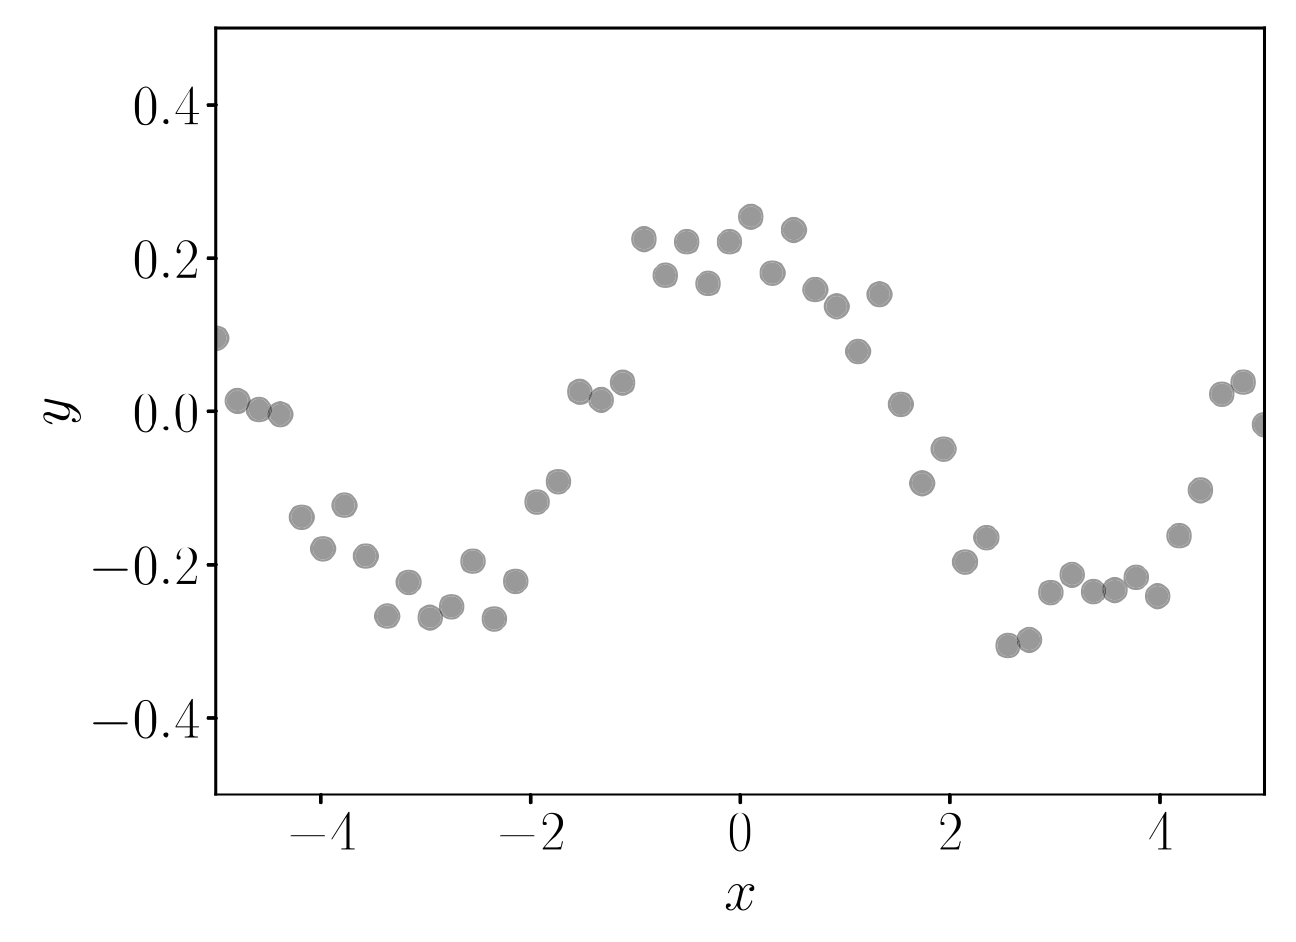
\includegraphics[width=0.5\linewidth]{polynomial_dataset}
\end{center}
Our goal is to find a function that is similar to the unknown function $f$
that generated the data. If we consider a standard linear regression,
represented as $f(x_n)=x_n^T\theta$, we can only fit straight lines to data.
However, if we consider the non linear transformation
$f(x_n)=\phi^T(x_n)\theta$, which is still linear in terms of $\theta$, we get
the corresponding linear model $y_i=\phi^T(x_n)\theta+\epsilon_i$ where
$\phi:\mathbb{R}^D\to \mathbb{R}^K$ and $\phi_k:\mathbb{R}^D\to \mathbb{R}$:
$$
\phi(x)=\begin{bmatrix}
    \phi_0(x) \\ 
    \phi_1(x) \\ 
    \vdots \\
    \phi_{K-1}(x)  
\end{bmatrix}
\in \mathbb{R}^K
$$
\begin{example}
    For a second polynomial the transformation $\phi(x)$ is defined as
    $$
    \phi=\begin{bmatrix}
        1 \\ 
        x \\ 
        x^2
    \end{bmatrix}
    $$    
\end{example}
The original one-dimensional space can be ``lifted" into a $K$-dimensional
feature space. If we choose all monomials $x^k$ for $k=0,\ldots,K-1$ we are
able to model polynomials $\leq K-1$ within the framework of linear
regression. A polynomial of degree $K-1$ is
$$
\begin{aligned}
    f(x_n)&=\phi^T(x_n)\theta \\
       &= \displaystyle\sum_{n=0}^{K-1}\theta_nx^n
\end{aligned}
$$
Considering all $N$ training inputs, we can define the \textit{feature matrix}
as 
$$
\Phi=\begin{bmatrix}
   \phi^T(x_1) \\ 
   \vdots \\
   \phi^T(x_N) 
\end{bmatrix} = \begin{bmatrix}
\phi_0^T(x_1) & \ldots & \phi_{K-1}(x_1) \\ 
\phi_0^T(x_2) & \ldots & \phi_{K-1}(x_2) \\
\vdots & & \vdots \\ 
\phi_0^T(x_N) & \ldots & \phi_{K-1}(x_N) \\
\end{bmatrix}
\in \mathbb{R}^{N\times K}
$$
where $\Phi_{ij}=\phi_j(x_i)$ and $\phi_j:\mathbb{R}^D\to \mathbb{R}$.
\begin{example}
    For a second-order polynomial and $N$ training points $x_n\in \mathbb{R}$,
    $n=1,\ldots,N$, the feature matrix is
    $$
    \Phi=\begin{bmatrix}
        1 & x_1 & x_1^2 \\ 
        1 & x_2 & x_2^2 \\ 
        \vdots & \vdots & \vdots \\ 
        1 & x_N & x_N^2
    \end{bmatrix}
    $$
\end{example}
With the feature matrix $\Phi$ defined, the negative log-likelihood for the
linear regression model can be written as 
$$-\log P_\theta(y|x)=\frac{1}{2\sigma^2}\lVert y-\Phi\theta\rVert^2$$
By treating the $\frac{1}{2\sigma^2}$ as a constant, the minimization problem
can be thought as least square problem:
$$\theta^*=\argmin_{\theta}\lVert y-\Phi\sigma\rVert^2$$
This least squares problem can be solved using the \textit{normal equations} or SGD:
$$
\begin{aligned}
    \min_x\lVert Ax-b\rVert^2 \\
    A^TAx-A^Tb=0 \\
    A^TAx=A^Tb \\ 
    x=(A^TA)^{-1}A^Tb
\end{aligned}
$$
Applying this to our minimization problem:
$$
\begin{aligned}
    \Phi^T\Phi\theta=\Phi^Ty\\
    \theta^*=(\Phi^T\Phi)^{-1}\Phi^Ty
\end{aligned}
$$
To get a better fit for our predictor, represented as
$f(x)=\sum_{n=0}^{K-1}\theta^*x^n$, on the training data, we can vary the
degree of the polynomial. 
\begin{center}
    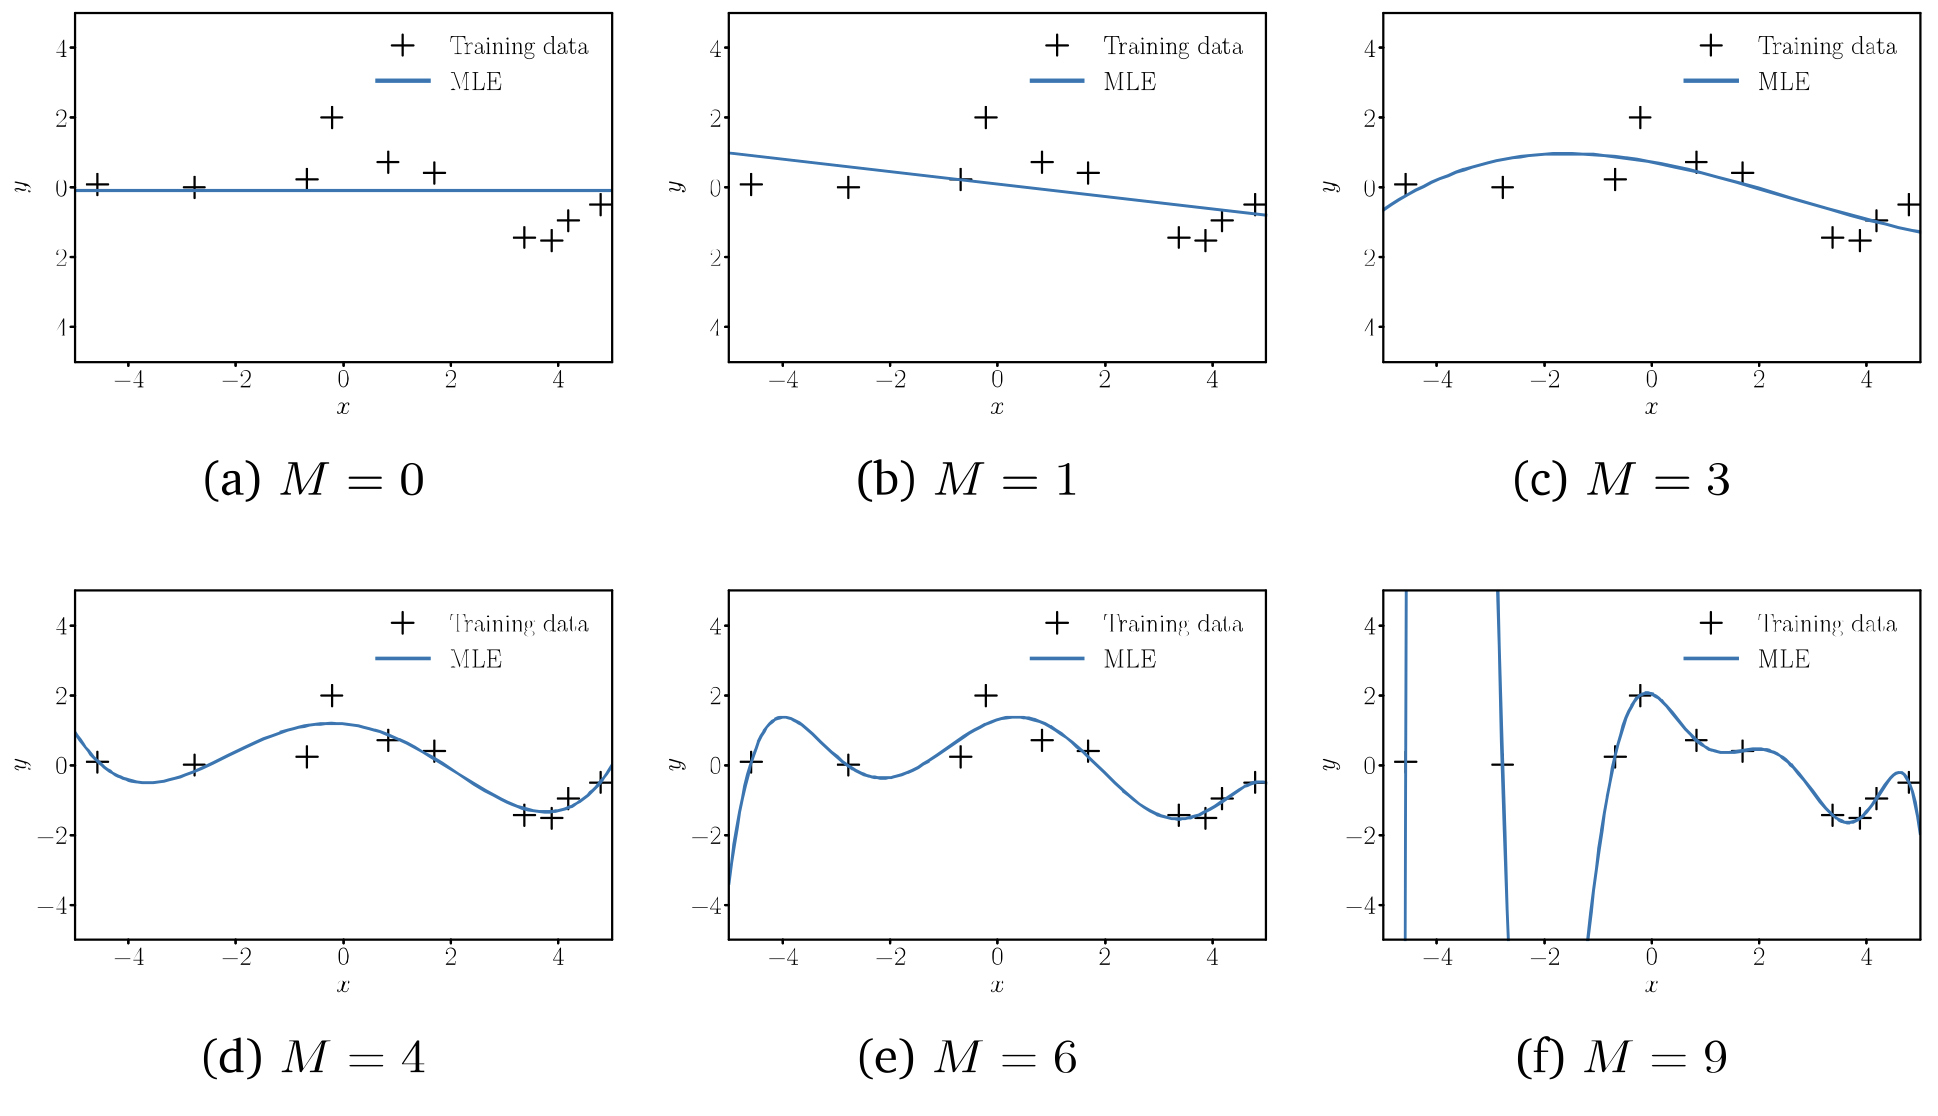
\includegraphics[width=\linewidth]{polynomial_degree}
\end{center}
However, our goal is to have a predictor that generalizes well. Therefore, we
plot the loss on both the training and test sets while varying the polynomial
degree.

A more robust metric for assessing the model's quality is by computing the
\textit{root mean square error (RMSE)}, defined as:
$$\sqrt{\lVert
y-\Phi\theta\rVert^2/N}=\sqrt{\frac{1}{N}\sum_{n=1}^{N}(y_n-\phi^T(x_n)\theta)^2}$$
which allows us to compare errors of dataset with different sizes and has the
same unit measure of the observed values $y_n$.

When observing that RMSE decreases on the training set but increases on the
test, it is indicative of overfitting. Again, we can plot the RMSE while
varying polynomial degree and opt for the higher one just before the
overfitting divergence happens.
\begin{center}
    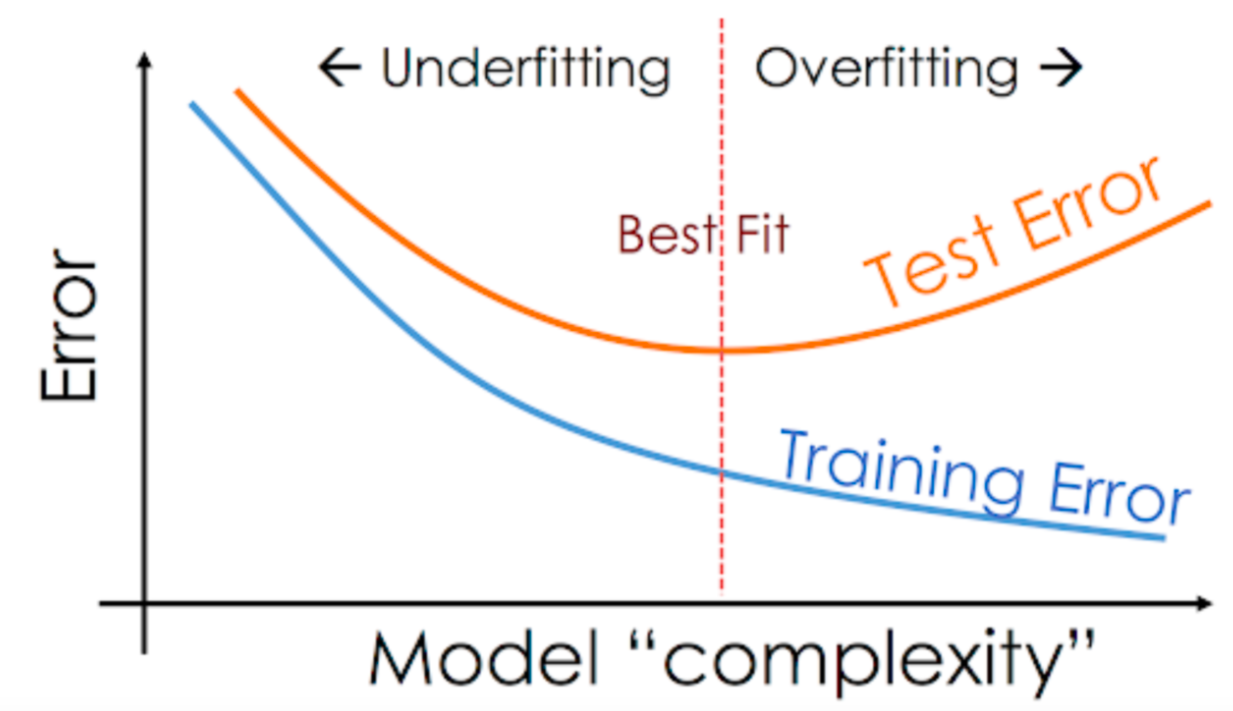
\includegraphics[width=0.75\linewidth]{overfit_underfit}
\end{center}
Another way to mitigate overfitting is through the use of regularization,
transitioning from MLE to MAP:
$$\theta^*=\argmin_\theta \lVert y-\Phi\theta\rVert^2+\lambda \lVert
\theta\rVert^2$$
\begin{center}
    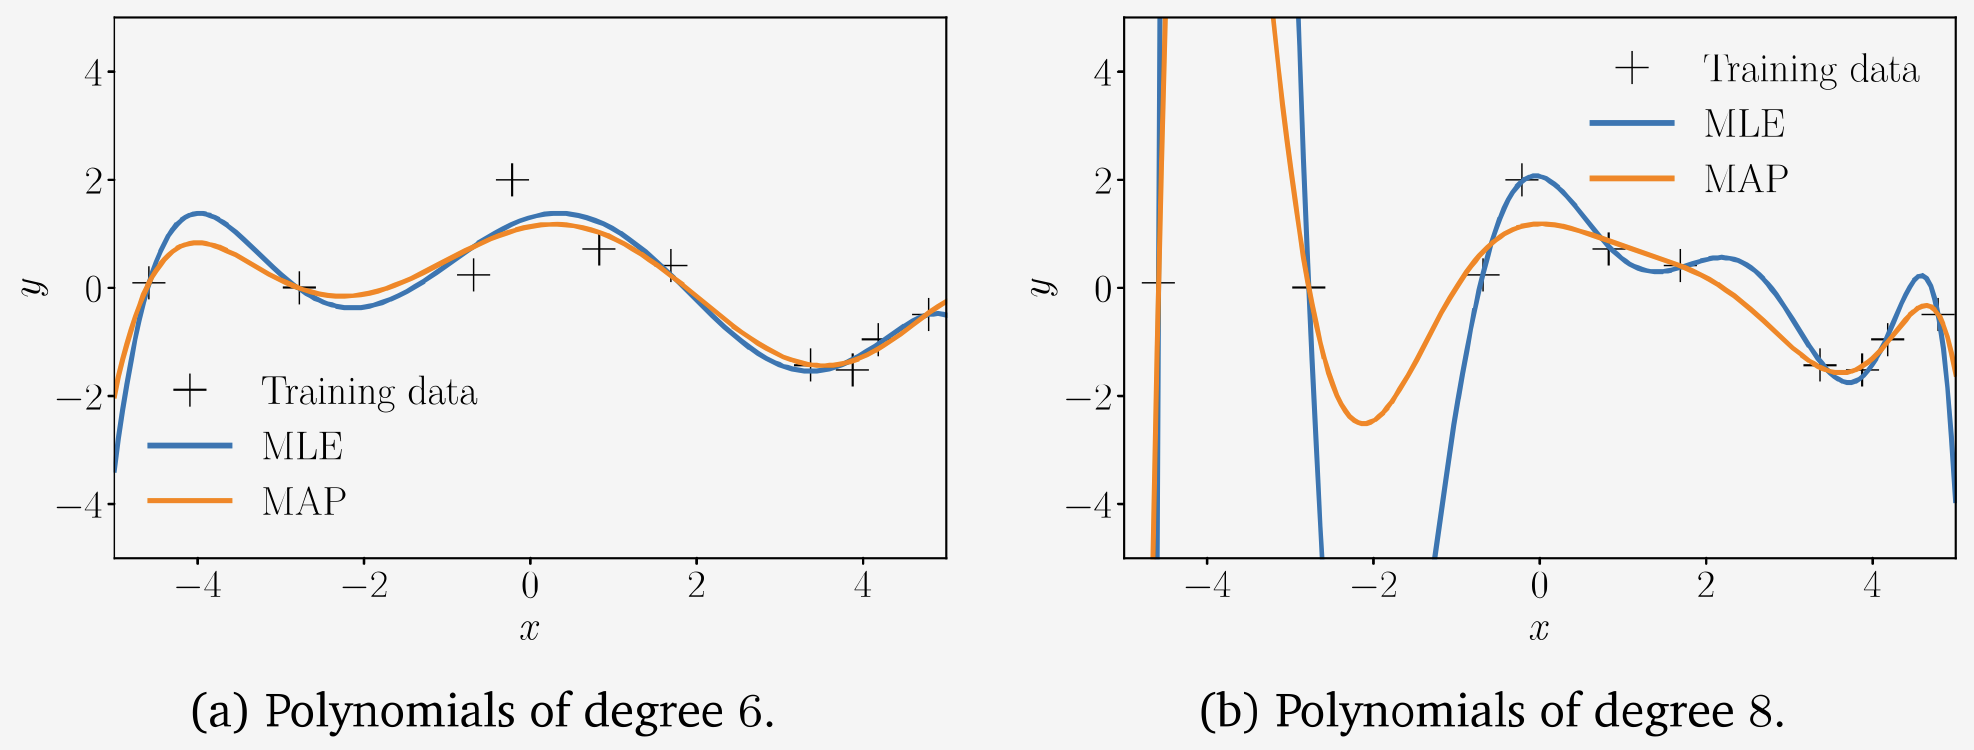
\includegraphics[width=\linewidth]{mle_map}
\end{center}
\end{document}
